%
% neldermead.tex --
%   Some notes about Nelder-Mead algorithms.
%
% Copyright 2008-2009 Michael Baudin
%
\documentclass[12pt]{report}

%% Good fonts for PDF
\usepackage[cyr]{aeguill}

%% Package for page headers
\usepackage{fancyhdr}

%% Package to include graphics
%% Comment for DVI
\usepackage[pdftex]{graphicx}

%% Index
\usepackage{makeidx}
\makeindex

%% Figures formats: jpeg or pdf
%% Comment for DVI
\DeclareGraphicsExtensions{.jpg,.pdf}

%% Package to create Hyperdocuments
%% Comment for DVI
\usepackage[pdftex,colorlinks=true,linkcolor=blue,citecolor=blue,urlcolor=blue]{hyperref}

%% Package to control printed area size
\usepackage{anysize}
%% ...by defining margins {left}{right}{top}{bottom}
\marginsize{22mm}{14mm}{12mm}{25mm}

%% Package used to include a bibliography
\usepackage{natbib}

%% R for real numbers
\usepackage{amssymb}

%% User defined commands

%% Figure reference
\newcommand{\figref}[1]{figure~\ref{#1}}

%% Equation reference
\newcommand{\Ref}[1]{(\ref{#1})}

%% Emphasize a word or a group of words
\newcommand{\empha}[1]{\textit{\textbf{#1}}}

%% Derivation operators
\newcommand{\D}{\partial}
\newcommand{\Dt}{\partial_t}
\newcommand{\Dx}{\partial_x}
\newcommand{\Dy}{\partial_y}

\newcommand{\bv}{\mathbf{v}}
\newcommand{\bx}{\mathbf{x}}
\newcommand{\bl}{\mathbf{l}}
\newcommand{\br}{\mathbf{r}}
\newcommand{\bg}{\mathbf{g}}

\usepackage{url}

% Scilab macros
\newcommand{\scifunction}[1]{\textit{#1}}

% To highlight source code
\usepackage{listings}

\lstdefinelanguage{scilabscript}%
  {morekeywords={abcd,abinv,abort,abs,acoshm,acosh,acosm,acos,addcolor,%
      addf,addinter,addmenu,add_edge,add_node,adj2sp,adj_lists,aff2ab,%
      amell,analpf,analyze,ans,apropos,arc_graph,arc_number,argn,arhnk,%
      arl2,arma2p,armac,armax1,armax,arma,arsimul,artest,articul,ascii,%
      asinhm,asinh,asinm,asin,atanhm,atanh,atanm,atan,augment,auread,%
      auwrite,balanc,balreal,bandwr,basename,bdiag,besseli,besselj,%
      besselk,bessely,best_match,bezout,bifish,bilin,binomial,black,%
      bloc2exp,bloc2ss,bode,bool2s,boolean,boucle,break,bstap,buttmag,%
      bvode,cainv,calerf,calfrq,call,canon,casc,case,ccontrg,cdfbet,%
      cdfbin,cdfchi,cdfchn,cdffnc,cdff,cdfgam,cdfnbn,cdfnor,cdfpoi,%
      cdft,ceil,center,cepstrum,chaintest,chain_struct,champ1,champ,%
      chart,chdir,cheb1mag,cheb2mag,check_graph,check_io,chepol,chfact,%
      chol,chsolve,circuit,classmarkov,clean,clearfun,clearglobal,%
      clear,close,cls2dls,cmb_lin,cmndred,cmoment,code2str,coeff,coffg,%
      coff,colcompr,colcomp,colinout,colormap,colregul,companion,comp,%
      cond,conj,connex,contour2di,contour2d,contourf,contour,%
      contract_edge,contrss,contr,cont_frm,cont_mat,convex_hull,convol,%
      convstr,con_nodes,copfac,copy,correl,corr,coshm,cosh,cosm,cos,%
      cotg,cothm,coth,covar,csim,cspect,ctr_gram,cumprod,cumsum,%
      curblock,cycle_basis,czt,c_link,dasrt,dassl,datafit,date,dbphi,%
      dcf,ddp,debug,dec2hex,deff,definedfields,degree,delbpt,%
      delete_arcs,delete_nodes,delete,delip,delmenu,demos,denom,%
      derivative,derivat,des2ss,des2tf,determ,detr,det,dft,dhinf,%
      dhnorm,diag,diary,diff,diophant,dirname,dispbpt,dispfiles,disp,%
      dlgamma,double,dragrect,drawaxis,drawlater,drawnow,draw,driver,%
      dscr,dsearch,dsimul,dtsi,dt_ility,duplicate,edge_number,%
      edit_curv,edit_graph_menus,edit_graph,edit,eigenmarkov,ell1mag,%
      elseif,else,emptystr,endfunction,end,eqfir,eqiir,equil1,equil,%
      ereduc,erfcx,erfc,erf,errbar,errcatch,errclear,error,eval3dp,%
      eval3d,eval,evans,evstr,excel2sci,execstr,exec,exists,exit,expm,%
      exp,external,eye,fac3d,factors,faurre,fchamp,fcontour2d,fcontour,%
      fec,feedback,feval,ffilt,fftshift,fft,fgrayplot,figure,fileinfo,%
      file,filter,findm,findobj,findx0BD,find_freq,find_path,find,%
      findABCD,findAC,findBD,findBDK,findR,fit_dat,fix,floor,flts,foo,%
      formatman,format,fort,for,fourplan,fplot2d,fplot3d1,fplot3d,%
      fprintf,fprintfMat,frep2tf,freq,freson,frexp,frfit,frmag,fscanf,%
      fscanfMat,fsfirlin,fsolve,fspecg,fstabst,fstair,ftest,ftuneq,%
      fullrfk,fullrf,full,fun2string,funcprot,functions,function,%
      funptr,fusee,gainplot,gamitg,gammaln,gamma,gcare,gcd,gcf,%
      genfac3d,genlib,genmarkov,gen_net,geom3d,geomean,getblocklabel,%
      getcolor,getcurblock,getcwd,getdate,getd,getenv,getfield,getfont,%
      getf,getio,getlinestyle,getmark,getpid,getscicosvars,getsymbol,%
      getvalue,getversion,get_function_path,get,gfare,gfrancis,girth,%
      givens,glever,glist,global,glue,gpeche,graduate,grand,%
      graphics_entities,graph_2_mat,graph_center,graph_complement,%
      graph_diameter,graph_power,graph_simp,graph_sum,graph_union,%
      graph-list,graycolormap,grayplot,graypolarplot,grep,group,%
      gr_menu,gschur,gsort,gspec,gstacksize,gtild,g_margin,h2norm,halt,%
      hamilton,hankelsv,hank,harmean,havewindow,help,hermit,hess,%
      hex2dec,hilb,hinf,hist3d,histplot,horner,host,hotcolormap,%
      householder,hrmt,htrianr,hypermat,h_cl,h_inf_st,h_inf,h_norm,%
      iconvert,icon_edit,ieee,if,iirgroup,iirlp,iir,ilib_build,%
      ilib_compile,ilib_for_link,ilib_gen_gateway,ilib_gen_loader,%
      ilib_gen_Make,imag,impl,imrep2ss,imult,im_inv,inistate,input,%
      int16,int2d,int32,int3d,int8,intc,intdec,integrate,interpln,%
      interp,intersci,intersect,intg,intl,intppty,intsplin,inttrap,%
      inttype,int,invr,invsyslin,inv_coeff,inv,iqr,isdef,isdir,isequal,%
      iserror,isglobal,isinf,isnan,isoview,isreal,is_connex,jmat,%
      justify,kalm,karmarkar,kernel,keyboard,knapsack,kpure,krac2,%
      kroneck,kron,lasterror,lattn,lattp,lcf,lcmdiag,lcm,ldivf,ldiv,%
      leastsq,legends,length,leqr,levin,lev,lex_sort,lft,lgfft,library,%
      lib,lin2mu,lincos,lindquist,lines,line_graph,linfn,linf,link,%
      linmeq,linpro,linsolve,linspace,lin,listfiles,list,lmisolver,%
      lmitool,loadmatfile,loadplots,loadwave,load_graph,load,locate,%
      log10,log1p,log2,logm,logspace,log,lotest,lqe,lqg2stan,lqg_ltr,%
      lqg,lqr,lsq,lsslist,lstcat,lstsize,ltitr,ludel,lufact,luget,%
      lusolve,lu,lyap,macglov,macr2lst,macrovar,macro,mad,make_graph,%
      make_index,manedit,man,mapsound,markp2ss,matfile2sci,matrix,%
      mat_2_graph,maxi,max_cap_path,max_clique,max_flow,max,mclearerr,%
      mclose,meanf,mean,median,meof,mese,mesh2d,mfft,mfile2sci,mgeti,%
      mgetl,mgetstr,mget,milk_drop,mine,mini,minreal,minss,%
      min_lcost_cflow,min_lcost_flow1,min_lcost_flow2,min_qcost_flow,%
      min_weight_tree,min,mlist,mode,modulo,moment,mopen,move,%
      mps2linpro,mputl,mputstr,mput,mrfit,msd,mseek,mtell,mtlb_load,%
      mtlb_mode,mtlb_save,mtlb_sparse,mu2lin,mulf,mvvacov,m_circle,%
      names,nand2mean,nanmax,nanmeanf,nanmean,nanmedian,nanmin,%
      nanstdev,nansum,narsimul,ndims,nearfloat,nehari,neighbors,%
      netclose,netwindows,netwindow,newest,newfun,nextpow2,nf3d,nfreq,%
      nlev,nnz,nodes_2_path,nodes_degrees,node_number,noisegen,norm,%
      null,numdiff,numer,nyquist,obscont1,obscont,observer,obsvss,%
      obsv_mat,obs_gram,odedc,odedi,odeoptions,ode_discrete,ode_root,%
      ode,oldload,oldsave,ones,optim,orth,param3d1,param3d,%
      paramfplot2d,parrot,part,pathconvert,path_2_nodes,pause,pbig,%
      pdiv,pen2ea,pencan,penlaur,perctl,perfect_match,pertrans,pfss,%
      phasemag,phc,pinv,pipe_network,playsnd,plot2d1,plot2d2,plot2d3,%
      plot2d4,plot2d,plot3d1,plot3d2,plot3d3,plot3d,plotframe,%
      plotprofile,plot_graph,plot,plzr,pmodulo,pol2des,pol2str,pol2tex,%
      polarplot,polar,polfact,poly,portr3d,portrait,power,ppol,prbs_a,%
      predecessors,predef,printf,printing,print,prod,profile,projsl,%
      projspec,proj,psmall,pspect,pvm_addhosts,pvm_barrier,pvm_bcast,%
      pvm_bufinfo,pvm_config,pvm_delhosts,pvm_error,pvm_exit,%
      pvm_f772sci,pvm_getinst,pvm_gettid,pvm_get_timer,pvm_gsize,%
      pvm_halt,pvm_joingroup,pvm_kill,pvm_lvgroup,pvm_mytid,pvm_parent,%
      pvm_probe,pvm_recv,pvm_reduce,pvm_sci2f77,pvm_send,pvm_set_timer,%
      pvm_spawn_independent,pvm_spawn,pvm_start,pvm_tasks,%
      pvm_tidtohost,pvm,pwd,p_margin,qassign,qr,quapro,quart,quaskro,%
      quit,randpencil,rand,range,rankqr,rank,rat,rcond,rdivf,read4b,%
      readb,readc_,readmps,read,real,recur,reglin,regress,remezb,remez,%
      repfreq,replot,residu,resume,return,riccati,riccsl,ricc,ric_desc,%
      rlist,roots,rotate,round,routh_t,rowcompr,rowcomp,rowinout,%
      rowregul,rowshuff,rpem,rref,rtitr,rubberbox,salesman,savewave,%
      save_graph,save,scaling,scanf,schur,sci2exp,sci2for,sci2map,%
      sciargs,scicosim,scicos,scifunc_block,sd2sci,secto3d,select,%
      semidef,sensi,setbpt,seteventhandler,setfield,setmenu,%
      setscicosvars,set,sfact,sgrid,shortest_path,showprofile,%
      show_arcs,show_graph,show_nodes,sident,signm,sign,simp_mode,simp,%
      sincd,sinc,sinc,sinhm,sinh,sinm,sin,size,sm2des,sm2ss,smooth,%
      solve,sorder,sort,sound,sp2adj,spaninter,spanplus,spantwo,sparse,%
      spchol,spcompack,specfact,spec,speye,spget,splin,split_edge,%
      spones,sprand,sprintf,spzeros,sqroot,sqrtm,sqrt,squarewave,%
      square,srfaur,srkf,ss2des,ss2ss,ss2tf,sscanf,sskf,ssprint,ssrand,%
      stabil,stacksize,standard_define,standard_draw,standard_input,%
      standard_origin,standard_output,startup,stdevf,stdev,steadycos,%
      str2code,strange,strcat,strindex,strings,string,stripblanks,%
      strong_connex,strong_con_nodes,strsubst,st_deviation,st_ility,%
      subf,subgraph,subplot,successors,sum,supernode,sva,svd,svplot,%
      sylm,sylv,sysconv,sysdiag,sysfact,syslin,syssize,systems,system,%
      systmat,tabul,tangent,tanhm,tanh,tanm,tan,tdinit,testmatrix,%
      texprint,tf2des,tf2ss,then,thrownan,timer,time_id,titlepage,%
      tk_getdir,tk_getfile,tlist,toeplitz,tokenpos,tokens,trace,%
      translatepaths,trans_closure,trans,trfmod,trianfml,tril,trimmean,%
      trisolve,triu,trzeros,typename,typeof,type,uicontrol,uimenu,%
      uint16,uint32,uint8,ui_observer,ulink,unglue,union,unique,unix_g,%
      unix_s,unix_w,unix_x,unix,unobs,unsetmenu,user,varargin,%
      varargout,variancef,variance,varn,warning,wavread,wavwrite,%
      wcenter,wfir,what,whereami,whereis,where,while,whos,who_user,who,%
      wiener,wigner,window,winsid,with_gtk,with_pvm,with_texmacs,%
      with_tk,writb,write4b,write,xarcs,xarc,xarrows,xaxis,xbasc,%
      xbasimp,xbasr,xchange,xclear,xclea,xclick,xclip,xdel,xend,xfarcs,%
      xfarc,xfpolys,xfpoly,xfrect,xgetech,xgetfile,xgetmouse,xget,%
      xgraduate,xgrid,xinfo,xinit,xlfont,xload,xname,xnumb,xpause,%
      xpolys,xpoly,xrects,xrect,xrpoly,xs2fig,xs2gif,xs2ppm,xs2ps,%
      xsave,xsegs,select,xsetech,xsetm,xset,xstringb,xstringl,xstring,%
      xtape,xtitle,x_choices,x_choose,x_dialog,x_matrix,x_mdialog,%
      x_message_modeless,x_message,yulewalk,zeropen,zeros,zgrid,zpbutt,%
      zpch1,zpch2,zpell,mfprintf,mfscanf,mprintf,mscanf,msprintf,%
      msscanf,mucomp,%
      ABSBLK_f,AFFICH_f,ANDLOG_f,ANIMXY_f,BIGSOM_f,CLINDUMMY_f,CLKIN_f,%
      CLKINV_f,CLKOUT_f,CLKOUTV_f,CLKSOM_f,CLKSOMV_f,CLKSPLIT_f,%
      CLOCK_f,CLR_f,CLSS_f,CONST_f,COSBLK_f,CURV_f,DELAY_f,DELAYV_f,%
      DEMUX_f,DLR_f,DLRADAPT_f,DLSS_f,EVENTSCOPE_f,EVTDLY_f,EVTGEN_f,%
      EXPBLK_f,G_make,GAIN_f,GAINBLK_f,GENERAL_f,GENERIC_f,GENSIN_f,%
      GENSQR_f,HALT_f,IFTHEL_f,IN_f,INTEGRAL_f,INTRP2BLK_f,INTRPLBLK_f,%
      INVBLK_f,LOGBLK_f,LOOKUP_f,Matplot1,Matplot,MAX_f,MCLOCK_f,%
      MFCLCK_f,MIN_f,MUX_f,NDcost,NEGTOPOS_f,OUT_f,POSTONEG_f,POWBLK_f,%
      PROD_f,QUANT_f,RAND_f,READC_f,REGISTER_f,RELAY_f,RFILE_f,%
      ScilabEval,Sfgrayplot,Sgrayplot,SAMPLEHOLD_f,SAT_f,SAWTOOTH_f,%
      SCOPE_f,SCOPXY_f,SELECT_f,SINBLK_f,SOM_f,SPLIT_f,STOP_f,SUPER_f,%
      TANBLK_f,TCLSS_f,TEXT_f,TIME_f,TK_EvalFile,TK_EvalStr,TK_GetVar,%
      TK_SetVar,TRASH_f,WFILE_f,WRITEC_f,ZCROSS_f,%
      \%asn,\%helps,\%k,\%sn},%
   alsoletter=\%,% chmod
   sensitive,%
   morecomment=[l]//,%
   morestring=[b]",%
   morestring=[m]'%
   numbers=none,%
   basicstyle=\tiny,%
   keywordstyle=\bfseries,%
   commentstyle=\bfseries,%
   showspaces=false,%
   stringstyle=\bfseries
  }[keywords,comments,strings]%

\lstdefinelanguage{matlabscript}%
  {morekeywords={gt,lt,gt,lt,amp,abs,acos,acosh,acot,acoth,acsc,acsch,%
      all,angle,ans,any,asec,asech,asin,asinh,atan,atan2,atanh,auread,%
      auwrite,axes,axis,balance,bar,bessel,besselk,bessely,beta,%
      betainc,betaln,blanks,bone,break,brighten,capture,cart2pol,%
      cart2sph,caxis,cd,cdf2rdf,cedit,ceil,chol,cla,clabel,clc,clear,%
      clf,clock,close,colmmd,Colon,colorbar,colormap,ColorSpec,colperm,%
      comet,comet3,compan,compass,computer,cond,condest,conj,contour,%
      contour3,contourc,contrast,conv,conv2,cool,copper,corrcoef,cos,%
      cosh,cot,coth,cov,cplxpair,cputime,cross,csc,csch,csvread,%
      csvwrite,cumprod,cumsum,cylinder,date,dbclear,dbcont,dbdown,%
      dbquit,dbstack,dbstatus,dbstep,dbstop,dbtype,dbup,ddeadv,ddeexec,%
      ddeinit,ddepoke,ddereq,ddeterm,ddeunadv,deblank,dec2hex,deconv,%
      del2,delete,demo,det,diag,diary,diff,diffuse,dir,disp,dlmread,%
      dlmwrite,dmperm,dot,drawnow,echo,eig,ellipj,ellipke,else,elseif,%
      end,engClose,engEvalString,engGetFull,engGetMatrix,engOpen,%
      engOutputBuffer,engPutFull,engPutMatrix,engSetEvalCallback,%
      engSetEvalTimeout,engWinInit,eps,erf,erfc,erfcx,erfinv,error,%
      errorbar,etime,etree,eval,exist,exp,expint,expm,expo,eye,fclose,%
      feather,feof,ferror,feval,fft,fft2,fftshift,fgetl,fgets,figure,%
      fill,fill3,filter,filter2,find,findstr,finite,fix,flag,fliplr,%
      flipud,floor,flops,fmin,fmins,fopen,for,format,fplot,fprintf,%
      fread,frewind,fscanf,fseek,ftell,full,function,funm,fwrite,fzero,%
      gallery,gamma,gammainc,gammaln,gca,gcd,gcf,gco,get,getenv,%
      getframe,ginput,global,gplot,gradient,gray,graymon,grid,griddata,%
      gtext,hadamard,hankel,help,hess,hex2dec,hex2num,hidden,hilb,hist,%
      hold,home,hostid,hot,hsv,hsv2rgb,if,ifft,ifft2,imag,image,%
      imagesc,Inf,info,input,int2str,interp1,interp2,interpft,inv,%
      invhilb,isempty,isglobal,ishold,isieee,isinf,isletter,isnan,%
      isreal,isspace,issparse,isstr,jet,keyboard,kron,lasterr,lcm,%
      legend,legendre,length,lin2mu,line,linspace,load,log,log10,log2,%
      loglog,logm,logspace,lookfor,lower,ls,lscov,lu,magic,matClose,%
      matDeleteMatrix,matGetDir,matGetFp,matGetFull,matGetMatrix,%
      matGetNextMatrix,matGetString,matlabrc,matlabroot,matOpen,%
      matPutFull,matPutMatrix,matPutString,max,mean,median,menu,mesh,%
      meshc,meshgrid,meshz,mexAtExit,mexCallMATLAB,mexdebug,%
      mexErrMsgTxt,mexEvalString,mexFunction,mexGetFull,mexGetMatrix,%
      mexGetMatrixPtr,mexPrintf,mexPutFull,mexPutMatrix,mexSetTrapFlag,%
      min,more,movie,moviein,mu2lin,mxCalloc,mxCopyCharacterToPtr,%
      mxCopyComplex16ToPtr,mxCopyInteger4ToPtr,mxCopyPtrToCharacter,%
      mxCopyPtrToComplex16,mxCopyPtrToInteger4,mxCopyPtrToReal8,%
      mxCopyReal8ToPtr,mxCreateFull,mxCreateSparse,mxCreateString,%
      mxFree,mxFreeMatrix,mxGetIr,mxGetJc,mxGetM,mxGetN,mxGetName,%
      mxGetNzmax,mxGetPi,mxGetPr,mxGetScalar,mxGetString,mxIsComplex,%
      mxIsFull,mxIsNumeric,mxIsSparse,mxIsString,mxIsTypeDouble,%
      mxSetIr,mxSetJc,mxSetM,mxSetN,mxSetName,mxSetNzmax,mxSetPi,%
      mxSetPr,NaN,nargchk,nargin,nargout,newplot,nextpow2,nnls,nnz,%
      nonzeros,norm,normest,null,num2str,nzmax,ode23,ode45,orient,orth,%
      pack,pascal,patch,path,pause,pcolor,pi,pink,pinv,plot,plot3,%
      pol2cart,polar,poly,polyder,polyeig,polyfit,polyval,polyvalm,%
      pow2,print,printopt,prism,prod,pwd,qr,qrdelete,qrinsert,quad,%
      quad8,quit,quiver,qz,rand,randn,randperm,rank,rat,rats,rbbox,%
      rcond,real,realmax,realmin,refresh,rem,reset,reshape,residue,%
      return,rgb2hsv,rgbplot,rootobject,roots,rose,rosser,rot90,rotate,%
      round,rref,rrefmovie,rsf2csf,save,saxis,schur,sec,sech,semilogx,%
      semilogy,set,setstr,shading,sign,sin,sinh,size,slice,sort,sound,%
      spalloc,sparse,spaugment,spconvert,spdiags,specular,speye,spfun,%
      sph2cart,sphere,spinmap,spline,spones,spparms,sprandn,sprandsym,%
      sprank,sprintf,spy,sqrt,sqrtm,sscanf,stairs,startup,std,stem,%
      str2mat,str2num,strcmp,strings,strrep,strtok,subplot,subscribe,%
      subspace,sum,surf,surface,surfc,surfl,surfnorm,svd,symbfact,%
      symmmd,symrcm,tan,tanh,tempdir,tempname,terminal,text,tic,title,%
      toc,toeplitz,trace,trapz,tril,triu,type,uicontrol,uigetfile,%
      uimenu,uiputfile,unix,unwrap,upper,vander,ver,version,view,%
      viewmtx,waitforbuttonpress,waterfall,wavread,wavwrite,what,%
      whatsnew,which,while,white,whitebg,who,whos,wilkinson,wk1read,%
      wk1write,xlabel,xor,ylabel,zeros,zlabel,zoom},%
   sensitive,%
   morecomment=[l]\%,%
   basicstyle=\tiny,%
   morestring=[m]'%
  }[keywords,comments,strings]%

\usepackage{algorithmic}

% To allow one bibliograph by chapter
%\usepackage[sectionbib]{chapterbib}
\usepackage{url}

% Maths shortcuts 
\newcommand{\RR}{\mathbb{R}}
\newcommand{\CC}{\mathbb{C}}

% For symbol degree
\DeclareTextSymbol{\degre}{T1}{6}





\begin{document}
%% User defined page headers
\pagestyle{fancyplain}
\renewcommand{\chaptermark}[1]{\markboth{\chaptername\ \thechapter. #1}{}}
\renewcommand{\sectionmark}[1]{\markright{\thesection. #1}}
\lhead[]{\fancyplain{}{\bfseries\leftmark}}
\rhead[]{\fancyplain{}{\bfseries\thepage}}
\cfoot{}

%% User defined figure legends
\makeatletter
\def\figurename{{\protect\sc \protect\small\bfseries Fig.}}
\def\f@ffrench{\protect\figurename\space{\protect\small\bf \thefigure}\space}
\let\fnum@figure\f@ffrench%
\let\captionORI\caption
\def\caption#1{\captionORI{\rm\small #1}}
\makeatother

%% First page
\thispagestyle{empty}
{
\begin{center}
%% Comment for DVI

\includegraphics[height=40mm]{scilab_logo}
\vskip2cm

%% Empty space between the box and the text
\fboxsep6mm
%% Box thickness
\fboxrule1.3pt
\Huge
$$\fbox{$
  \begin{array}{c}
  \textbf{Nelder-Mead}\\
  \textbf{User's Manual}\\
  \textbf{-- The Nelder-Mead Method --}\\
  \end{array}
  $}
$$
\end{center}

\vskip1cm

\begin{center}
\begin{large}
Micha\"el BAUDIN
\end{large}
\end{center}

\vskip2cm


\vskip1cm


\begin{flushright}
Version 0.3 \\
September 2009
\end{flushright}



\clearpage

%% Table of contents
\renewcommand{\baselinestretch}{1.30}\small \normalsize

\tableofcontents

\renewcommand{\baselinestretch}{1.18}\small \normalsize

\chapter*{Notations}


\begin{figure}[h]
\begin{center}
\begin{tabular}{|l|l|}
\hline
$n$ & number of variables\\
$\bx=(x_1,x_2,\ldots,x_n)^T \in\RR^n$ & the unknown\\
$\bx_0\in\RR^n$ & the initial guess\\
$\bv\in\RR^n$ & a vertex\\
$S=\{\bv_i\}_{i=1,m}$ & a complex, where $m\geq n+1$ is the number of vertices\\
$S=\{\bv_i\}_{i=1,n+1}$ & a simplex (with $n+1$ vertices)\\
$(\bv_i)_j$ & the $j$-th component of the $i$-th vertex\\
$S_0$& the initial simplex\\
$S_k$& the simplex at iteration $k$\\
$f:\RR^n\rightarrow\RR$& the cost function\\
\hline
\end{tabular}
\end{center}
\caption{Notations used in this document}
\label{fig-notations}
\end{figure}

\chapter{Nelder-Mead method}

In this chapter, we present Nelder and Mead's \cite{citeulike:3009487} algorithm.
We begin by the analysis of the algorithm, which is based on a variable shape simplex.
Then, we present geometric situations where the various steps of the algorithm 
are used. In the third part, we present the rate of convergence toward the optimum of 
the Nelder-Mead algorithm. This part is mainly based on Han and Neumann's paper \cite{HanNeumann2006}, 
which makes use of a class of quadratic functions with a special initial 
simplex. The core of this chapter is the analysis of several numerical 
experiments which have been performed with the neldermead component.
We analyze the behavior of the algorithm on quadratic functions and 
present several counter examples where the Nelder-Mead algorithm is 
known to fail.

\section{Introduction}

In this section, we present the Nelder-Mead algorithm for unconstrained optimization.
This algorithm is based on the iterative update of a simplex. 
Then we present various geometric situations which might occur
during the algorithm. 

\subsection{Overview}

The goal of the Nelder and Mead algorithm is to solve the 
following unconstrained optimization problem
\begin{eqnarray}
\min f(\bx)
\end{eqnarray}
where $\bx\in \RR^n$, $n$ is the number of optimization parameters and $f$ is the objective 
function $f:\RR^n\rightarrow \RR$.

The Nelder-Mead method is an improvement over the Spendley's et al.
method with the goal of allowing the simplex to vary in \emph{shape}, 
and not only in \emph{size}, as in Spendley's et al. algorithm.

This algorithms is based on the iterative update of 
a \emph{simplex} made of $n+1$ points $S=\{\bv_i\}_{i=1,n+1}$. Each point 
in the simplex is called a \emph{vertex} and is associated with 
a function value $f_i=f(\bv_i)$ for $i=1,n+1$.

The vertices are sorted by increasing function values so that the 
\emph{best} vertex has index 1 and the \emph{worst} vertex 
has index $n+1$
\begin{eqnarray}
\label{sorted-vertices-fv}
f_1 \leq f_2 \leq \ldots \leq f_n \leq f_{n+1}.
\end{eqnarray}

The $\bv_1$ vertex (resp. the $\bv_{n+1}$ vertex) is called the \emph{best} 
vertex (resp. \emph{worst}), because it is associated with the lowest (resp. highest)
function value. 

The centroid of the simplex $\overline{\bx} (j)$ is the center of the vertices
where the vertex $\bv_j$ has been 
excluded. This centroid is 
\begin{eqnarray}
\label{centroid-generalized}
\overline{\bx} (j) = 
\frac{1}{n} \sum_{i=1,n+1, i\neq j} \bv_i.
\end{eqnarray}
The algorithm makes use
of one coefficient $\rho>0$, called the reflection factor. The standard
value of this coefficient is $\rho=1$.
The algorithm attempts to replace some vertex 
$\bv_j$ by a new vertex $\bx(\rho,j)$ on the line from the vertex $\bv_j$
to the centroid  $\overline{\bx}(j)$. The new vertex $\bx(\rho,j)$ is defined by 
\begin{eqnarray}
\label{interpolate-generalized}
\bx(\rho,j) = (1+\rho)\overline{\bx}(j) - \rho \bv_j.
\end{eqnarray}

\subsection{Algorithm}

In this section, we analyze the Nelder-Mead algorithm, which
is presented in figure \ref{algo-neldermead}.

\begin{figure}[htbp]
\begin{algorithmic}
\STATE Compute an initial simplex $S_0$
\STATE Sorts the vertices $S_0$ with increasing function values
\STATE $S\gets S_0$
\WHILE{$\sigma(S)>tol$}
  \STATE $\overline{x}\gets \overline{x}(n+1)$
  \STATE $x_r \gets x(\rho,n+1)$ \COMMENT{Reflect}
  \STATE $f_r \gets f(x_r)$ 
  \IF {$f_r<f_1$}
    \STATE $x_e \gets x(\rho\chi,n+1)$ \COMMENT{Expand}
    \STATE $f_e \gets f(x_e)$ 
    \IF {$f_e<f_r$}
      \STATE Accept $x_e$
    \ELSE
      \STATE Accept $x_r$
    \ENDIF
  \ELSIF {$f_1 \leq f_r < f_n$}
    \STATE Accept $x_r$
  \ELSIF {$f_n \leq f_r < f_{n+1}$}
    \STATE $x_c \gets x(\rho\gamma,n+1)$ \COMMENT{Outside contraction}
    \STATE $f_c \gets f(x_c)$ 
    \IF {$f_c<f_r$}
      \STATE Accept $x_c$
    \ELSE
      \STATE Compute the points $x_i=x_1 + \sigma (x_i - x_1)$, $i=2,n+1$ \COMMENT{Shrink}
      \STATE Compute $f_i = f(\bv_i)$ for $i=2,n+1$
    \ENDIF
  \ELSE
    \STATE $x_c \gets x(-\gamma,n+1)$ \COMMENT{Inside contraction}
    \STATE $f_c \gets f(x_c)$ 
    \IF {$f_c<f_{n+1}$}
      \STATE Accept $x_c$
    \ELSE
      \STATE Compute the points $x_i=x_1 + \sigma (x_i - x_1)$, $i=2,n+1$ \COMMENT{Shrink}
      \STATE Compute $f_i = f(\bv_i)$ for $i=2,n+1$
    \ENDIF
  \ENDIF
  \STATE Sort the vertices of $S$ with increasing function values
\ENDWHILE
\end{algorithmic}
\caption{Nelder-Mead algorithm -- Standard version}
\label{algo-neldermead}
\end{figure}

The Nelder-Mead algorithm makes use of four parameters: the 
coefficient of reflection $\rho$, expansion $\chi$, 
contraction $\gamma$ and shrinkage $\sigma$.
When the expansion or contraction steps are performed, the shape 
of the simplex is changed, thus "adapting itself to the 
local landscape" \cite{citeulike:3009487}.

These parameters should satisfy the following inequalities \cite{citeulike:3009487,lagarias:112}
\begin{eqnarray}
\label{condition-coeffs}
\rho>0, \qquad \chi > 1, \qquad \chi > \rho, \qquad 0<\gamma<1 \qquad \textrm{and} \qquad 0<\sigma<1.
\end{eqnarray}
The standard values for these coefficients are 
\begin{eqnarray}
\label{standard-coeffs}
\rho=1, \qquad \chi =2, \qquad \gamma=\frac{1}{2} \qquad \textrm{and} \qquad \sigma=\frac{1}{2}.
\end{eqnarray}

In \cite{Kelley1999}, the Nelder-Mead algorithm is presented with 
other parameter names, that is $\mu_r = \rho$, $\mu_e = \rho\chi$, $\mu_{ic} = -\gamma$
and $\mu_{oc} = \rho\gamma$. These coefficients must satisfy the following 
inequality 
\begin{eqnarray}
-1 < \mu_{ic} < 0 < \mu_{oc} < \mu_r < \mu_e.
\end{eqnarray}

At each iteration, we compute the centroid 
$\overline{\bx} (n+1)$ where the worst vertex $\bv_{n+1}$ 
has been excluded. This centroid is 
\begin{eqnarray}
\label{centroid-worst}
\overline{\bx} (n+1) = \frac{1}{n} \sum_{i=1,n} \bv_i.
\end{eqnarray}
We perform a reflection with respect to the worst vertex $\bv_{n+1}$,
which creates the reflected point $\bx_r$ defined by 
\begin{eqnarray}
\label{interpolate-worst}
\bx_r = \bx(\rho,n+1) = (1+\rho)\overline{\bx}(n+1) - \rho \bv_{n+1}
\end{eqnarray}
We then compute the function value of the reflected
point as $f_r=f(\bx_r)$. 

From that point, there are several possibilities, which 
are listed below. Most steps try to replace the 
worst vertex $\bv_{n+1}$ by a better point, which is computed 
depending on the context.
\begin{itemize}
\item In the case where $f_r<f_1$, the reflected point $\bx_r$
were able to improve (i.e. reduce) the function value. In that case, the algorithm
tries to expand the simplex so that the function value is improved 
even more. The expansion point is computed by 
\begin{eqnarray}
\bx_e = \bx(\rho\chi,n+1) = (1+\rho\chi)\overline{\bx}(n+1) - \rho\chi \bv_{n+1}
\end{eqnarray}
and the function is computed at this point, i.e. we compute 
$f_e = f(\bx_e)$.
If the expansion point allows to improve the function 
value, the worst vertex 
$\bv_{n+1}$ is rejected from the simplex and the expansion point $\bx_e$
is accepted. If not, the reflection point $\bx_r$ is accepted.
\item In the case where $f_1\leq f_r<f_n$, the worst vertex 
$\bv_{n+1}$ is rejected from the simplex and the reflected point $\bx_r$
is accepted.
\item In the case where $f_n\leq f_r<f_{n+1}$, we consider the point 
\begin{eqnarray}
\bx_c = \bx(\rho\gamma,n+1) = (1+\rho\gamma)\overline{\bx}(n+1) - \rho\gamma \bv_{n+1}
\end{eqnarray}
is considered. If the point $\bx_c$ is better than the reflection point $\bx_r$,
then it is accepted. If not, a shrink step is performed, where 
all vertices are moved toward the best vertex $\bv_1$.
\item In other cases, we consider the point 
\begin{eqnarray}
\bx_c = \bx(-\gamma,n+1) = (1-\gamma)\overline{\bx}(n+1) + \gamma \bv_{n+1}.
\end{eqnarray}
If the point $\bx_c$ is better than the worst vertex $\bx_{n+1}$,
then it is accepted. If not, a shrink step is performed.
\end{itemize}

The algorithm from figure \ref{algo-neldermead} is the most 
popular variant of the Nelder-Mead algorithm.
But the original paper is based on a "greedy" expansion, where 
the expansion point is accepted if it is better than the 
best point (and not if it is better than the reflection point).
This "greedy" version is implemented in AS47 by O'Neill in \cite{O'Neill1971AAF}
and the corresponding algorithm is presented in figure \ref{algo-neldermead-greedy}.

\begin{figure}[htbp]
\begin{verbatim}
[...]
\end{verbatim}
\begin{algorithmic}
    \STATE $\bx_e \gets \bx(\rho\chi,n+1)$ \COMMENT{Expand}
    \STATE $f_e \gets f(\bx_e)$ 
    \IF {$f_e<f_1$}
      \STATE Accept $\bx_e$
    \ELSE
      \STATE Accept $\bx_r$
    \ENDIF
\end{algorithmic}
\begin{verbatim}
[...]
\end{verbatim}
\caption{Nelder-Mead algorithm -- Greedy version}
\label{algo-neldermead-greedy}
\end{figure}


\section{Geometric analysis}

The figure \ref{fig-nm-moves} presents the various moves of the 
simplex in the Nelder-Mead algorithm.

\begin{figure}
\begin{center}
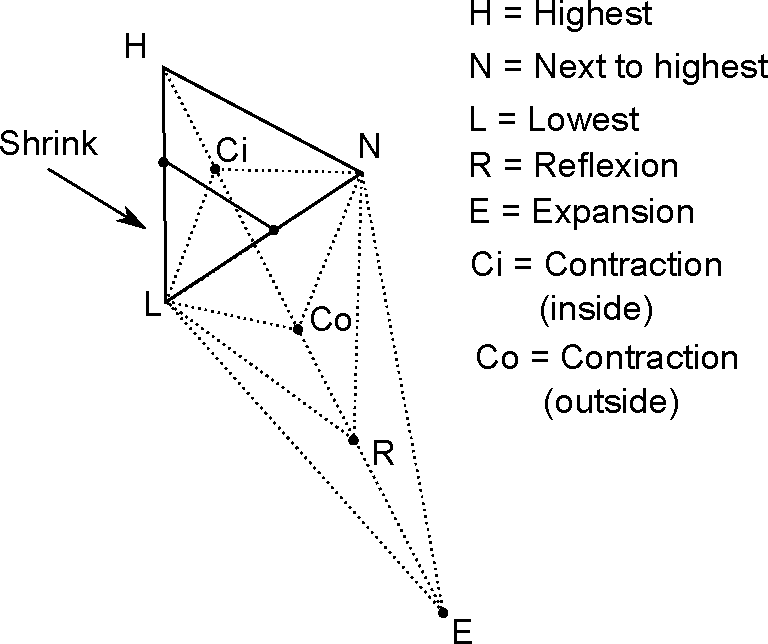
\includegraphics[width=6cm]{nelder-mead-steps.pdf}
\end{center}
\caption{Nelder-Mead simplex steps}
\label{fig-nm-moves}
\end{figure}

The figure \ref{fig-nm-moves-reflection} 
to \ref{fig-nm-moves-shrinkafterco} present the 
detailed situations when each type of step occur.
We emphasize that these figures are not the result of 
numerical experiments. These figures been created in order 
to illustrate specific points of the algorithm.

\begin{itemize}
\item Obviously, the expansion step is performed when the 
simplex is far away from the optimum. The direction of 
descent is then followed and the worst vertex is moved 
into that direction.
\item When the reflection step is performed, the simplex is 
getting close to an valley, since the expansion point 
does not improve the function value.
\item When the simplex is near the optimum, 
the inside and outside contraction steps may be performed, which 
allows to decrease the size of the simplex.
The figure \ref{fig-nm-moves-insidecontraction}, which illustrates 
the inside contraction step, happens in "good" situations.
As presented in section \ref{section-mcKinnon}, applying 
repeatedly the inside contraction step can transform 
the simplex into a degenerate simplex, which may let the algorithm
converge to a non stationnary point.
\item The shrink steps (be it after an outside contraction or an inside 
contraction) occurs only in very special situations. In practical experiments,
shrink steps are rare.
\end{itemize}

\begin{figure}
\begin{center}
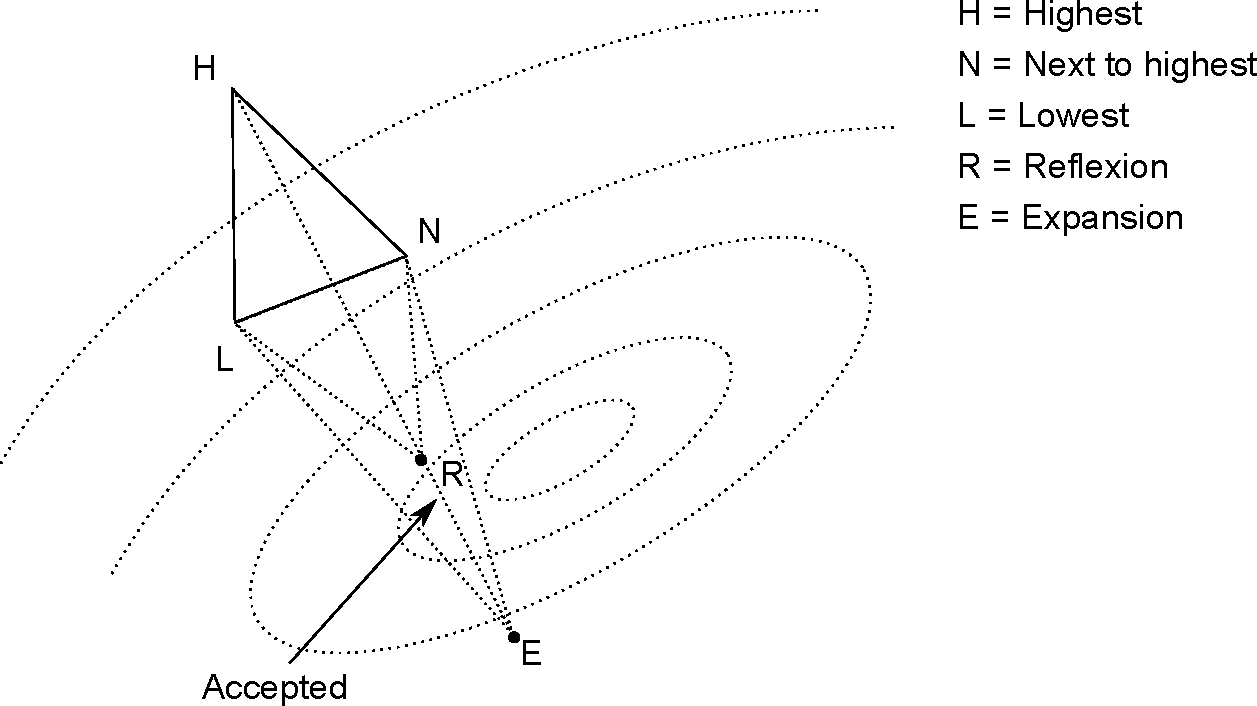
\includegraphics[width=10cm]{nelder-mead-reflection.pdf}
\end{center}
\caption{Nelder-Mead simplex moves -- Reflection}
\label{fig-nm-moves-reflection}
\end{figure}

\begin{figure}
\begin{center}
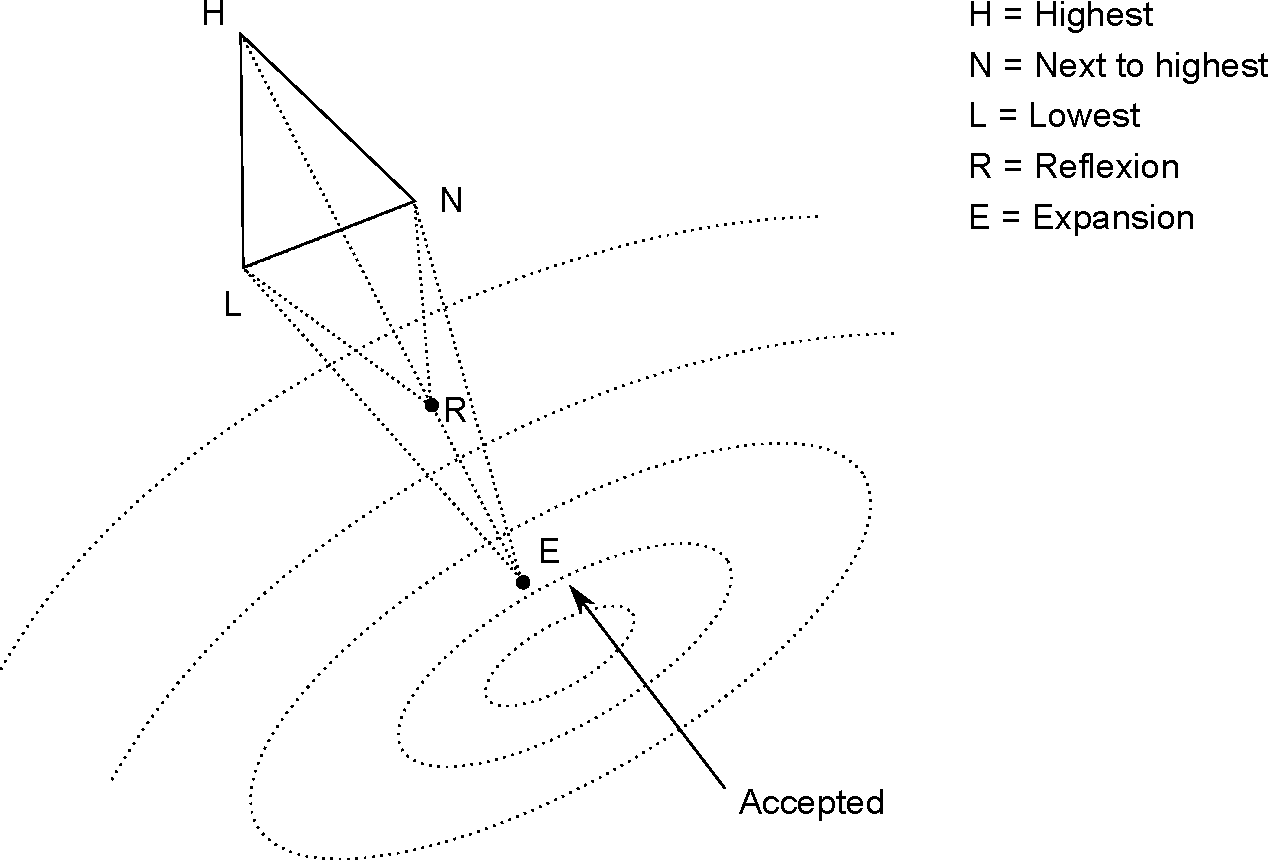
\includegraphics[width=10cm]{nelder-mead-extension.pdf}
\end{center}
\caption{Nelder-Mead simplex moves -- Expansion}
\label{fig-nm-moves-expansion}
\end{figure}

\begin{figure}
\begin{center}
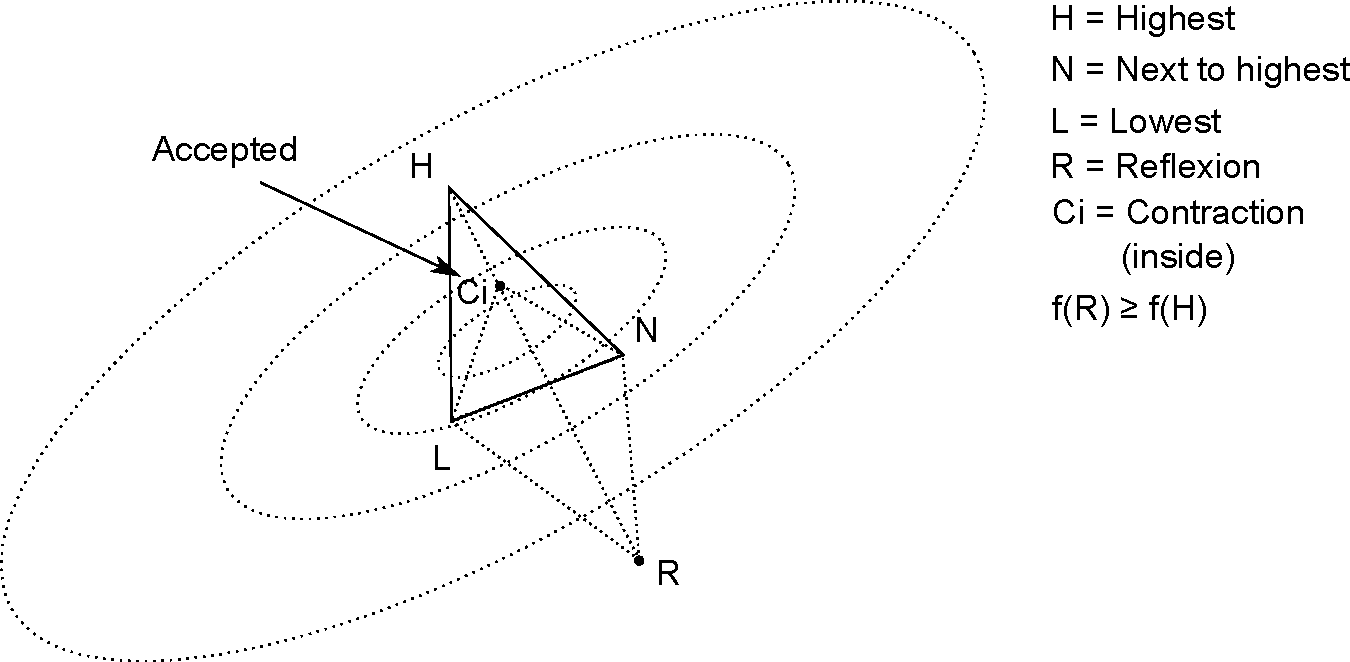
\includegraphics[width=10cm]{nelder-mead-contract-inside.pdf}
\end{center}
\caption{Nelder-Mead simplex moves - Inside contraction}
\label{fig-nm-moves-insidecontraction}
\end{figure}

\begin{figure}
\begin{center}
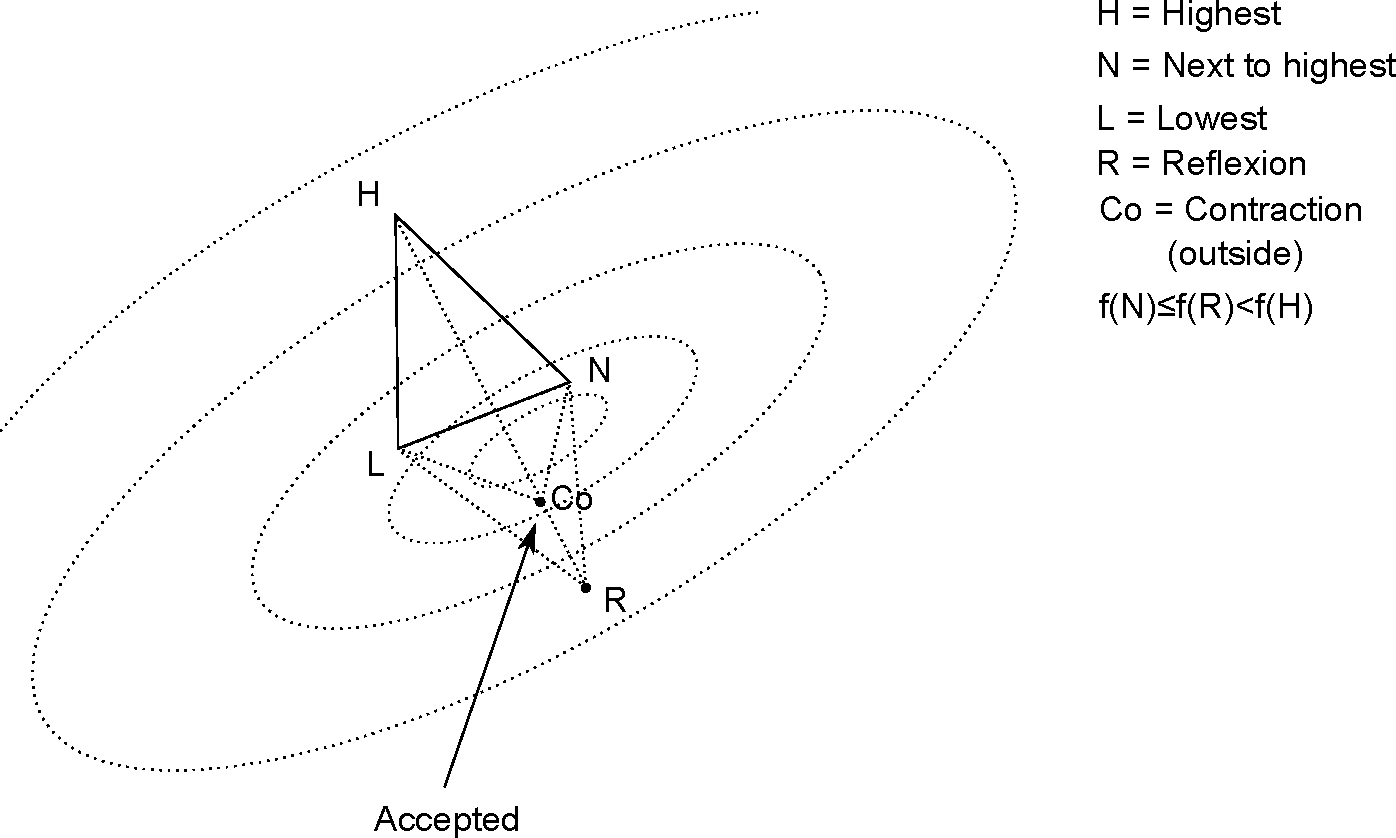
\includegraphics[width=10cm]{nelder-mead-contract-outside.pdf}
\end{center}
\caption{Nelder-Mead simplex moves -- Outside contraction}
\label{fig-nm-moves-outsidecontraction}
\end{figure}

\begin{figure}
\begin{center}
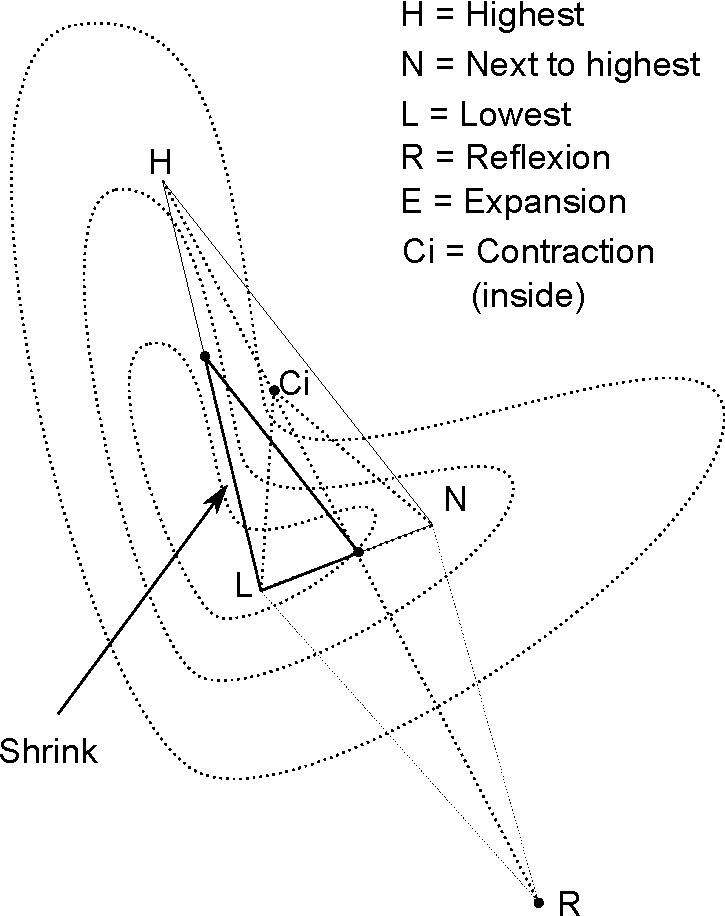
\includegraphics[width=6cm]{nelder-mead-shrink-afterci.pdf}
\end{center}
\caption{Nelder-Mead simplex moves -- Shrink after inside contraction.}
\label{fig-nm-moves-shrinkafterci}
\end{figure}

\begin{figure}
\begin{center}
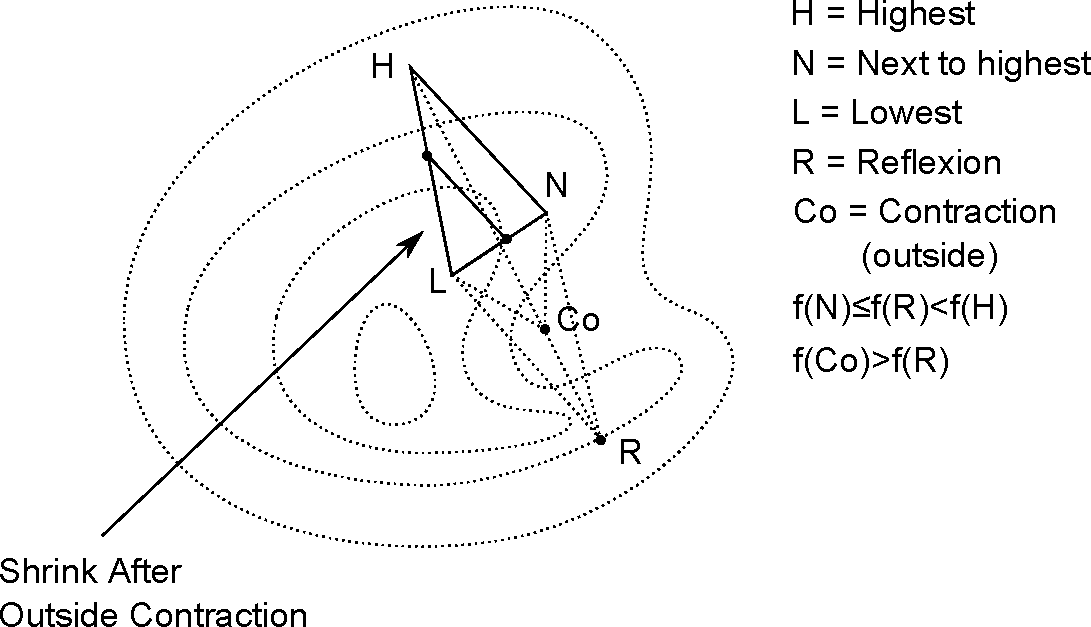
\includegraphics[width=10cm]{nelder-mead-shrink-afterco.pdf}
\end{center}
\caption{Nelder-Mead simplex moves -- Shrink after outside contraction}
\label{fig-nm-moves-shrinkafterco}
\end{figure}


%\subsection{Termination criteria}

%TODO...

\section{Convergence properties on a quadratic}

In this section, we reproduce one result 
presented by Han and Neumann \cite{HanNeumann2006}, which states 
the rate of convergence toward the optimum on a class of quadratic 
functions with a special initial simplex.
Some additional results are also presented in the Phd thesis by Lixing Han \cite{Han2000}.
We study a generalized quadratic and use a particular 
initial simplex. We show that the vertices follow 
a recurrence equation, which is associated with a characteristic 
equation. The study of the roots of these characteristic equations 
give an insight of the behavior of the Nelder-Mead algorithm
when the dimension $n$ increases.

Let us suppose than we want to minimize the function 
\begin{eqnarray}
\label{hanneumman-quadratic}
f(\bx) = x_1^2+\ldots+x_n^2
\end{eqnarray}
with the initial simplex 
\begin{eqnarray}
S_0 = \left[\bold{0},\bv^{(0)}_1,\ldots,\bv^{(0)}_n\right]
\end{eqnarray}
With this choice of the initial simplex, the best vertex remains fixed 
at $\bold{0}=(0,0,\ldots,0)^T\in\RR^n$. As the cost function \ref{hanneumman-quadratic}
is strictly convex, the Nelder-Mead method never performs
the \emph{shrink} step. Therefore, at each iteration, a new simplex 
is formed by replacing the worst vertex $\bv^{(k)}_n$, by a 
new, better vertex. Assume that the Nelder-Mead method 
generates a sequence of simplices $\{S_k\}_{k\geq 0}$ in $\RR^n$,
where 
\begin{eqnarray}
S_k = \left[\bold{0},\bv^{(k)}_1,\ldots,\bv^{(n)}_n\right]
\end{eqnarray}
We wish that the sequence of simplices $S_k\rightarrow \bold{0}\in\RR^n$
as $k\rightarrow \infty$. To measure the progress of convergence,
Han and Neumann use the oriented length $\sigma_+(S_k)$ of the simplex $S_k$,
defined by 
\begin{eqnarray}
\sigma_+(S) = \max_{i=2,m} \|\bv_i - \bv_1\|_2.
\end{eqnarray}
We say that a sequence of simplices $\{S_k\}_{k\geq 0}$ converges to the minimizer $\bold{0}\in\RR^n$
of the function in equation \ref{hanneumman-quadratic} if 
$\lim_{k\rightarrow \infty} \sigma_+(S_k) = 0$.

We measure the rate of convergence defined by 
\begin{eqnarray}
\label{rho-rate-convergence}
\rho(S_0,n) = \textrm{lim sup}_{k\rightarrow \infty} 
\left(\sum_{i=0,k-1} \frac{\sigma(S_{i+1})}{\sigma(S_i)}\right)^{1/k}
\end{eqnarray}
That definition can be viewed as the geometric mean of the ratio of the 
oriented lengths between successive simplices and the minimizer 0.
This definition implies 
\begin{eqnarray}
\label{rho-rate-convergence2}
\rho(S_0,n) = \textrm{lim sup}_{k\rightarrow \infty} 
\left( \frac{\sigma(S_{k+1})}{\sigma(S_0)}\right)^{1/k}
\end{eqnarray}

According to the definition, the algorithm is convergent if $\rho(S_0,n) < 1$.
The larger the $\rho(S_0,n)$, the slower the convergence. In particular, the convergence 
is very slow when $\rho(S_0,n)$ is close to 1. 
The analysis is based on the fact that the Nelder-Mead method generates a sequence of simplices
in $\RR^n$ satisfying 
\begin{eqnarray}
S_k = \left[\bold{0},\bv^{(k+n-1)},\ldots,\bv^{(k+1)},\bv^{(k)}\right],
\end{eqnarray}
where $\bold{0},\bv^{(k+n-1)},\ldots,\bv^{(k+1)},\bv^{(k)}\in\RR^n$ are the vertices
of the $k-th$ simplex, with
\begin{eqnarray}
f(\bold{0}) < f\left(\bv^{(k+n-1)}\right) < f\left(\bv^{(k+1)}\right) < f\left(\bv^{(k)}\right),
\end{eqnarray}
for $k\geq 0$. 

To simplify the analysis, we consider that only one type of step of the Nelder-Mead 
method is applied repeatedly. This allows to establish recurrence equations for the 
successive simplex vertices. As the shrink step is never used, and the expansion steps is 
never used neither (since the best vertex is already at 0), the analysis focuses
on the outside contraction, inside contraction and reflection steps.

The centroid of the $n$ best vertices of $S_k$ is given by 
\begin{eqnarray}
\overline{\bold{v}}^{(k)} 
&=&\frac{1}{n} \left( \bv^{(k+1)} + \ldots + \bv^{(k+n-1)} + \bold{0} \right)\\
&=&\frac{1}{n} \left( \bv^{(k+1)} + \ldots + \bv^{(k+n-1)} \right)\\
&=& \frac{1}{n} \sum_{i=1,n-1} \bv^{(k+i)} \label{eq-nm-centroid}
\end{eqnarray}

\subsection{With default parameters}

In this section, we analyze the roots of the characteristic 
equation with \emph{fixed}, standard inside and outside contraction
coefficients.

\emph{Outside contraction} \\
If the outside contraction step is repeatedly performed
with $\mu_{oc} = \rho\gamma = \frac{1}{2}$, then 
\begin{eqnarray}
\bv^{(k+n)} = \overline{\bold{v}}^{(k)} 
+ \frac{1}{2} \left( \overline{\bold{v}}^{(k)} - \bv^{(k)}\right) .
\end{eqnarray}
By plugging the definition of the centroid \ref{eq-nm-centroid} into the previous equality, we 
find the recurrence formula
\begin{eqnarray}
2n \bv^{(k+n)} - 3 \bv^{(k+1)} - \ldots - 3 \bv^{(k+n-1)} + n\bv^{(k)} = 0.
\end{eqnarray}
The associated characteristic equation is 
\begin{eqnarray}
\label{recurrence-oc}
2n \mu^n - 3 \mu^{n-1} - \ldots - 3 \mu + n = 0.
\end{eqnarray}

\emph{Inside contraction} \\
If the inside contraction step is repeatedly performed
with $\mu_{ic} = -\gamma = -\frac{1}{2}$, then 
\begin{eqnarray}
\bv^{(k+n)} = \overline{\bold{v}}^{(k)} 
- \frac{1}{2} \left( \overline{\bold{v}}^{(k)} - \bv^{(k)}\right).
\end{eqnarray}
By plugging the definition of the centroid \ref{eq-nm-centroid} into the previous equality, we 
find the recurrence formula
\begin{eqnarray}
2n \bv^{(k+n)} - \bv^{(k+1)} - \ldots - \bv^{(k+n-1)} - n\bv^{(k)} = 0.
\end{eqnarray}
The associated characteristic equation is 
\begin{eqnarray}
\label{recurrence-ic}
2n \mu^n - \mu^{n-1} - \ldots - \mu - n = 0.
\end{eqnarray}

\emph{Reflection}  \\
If the reflection step is repeatedly performed
with $\mu_r = \rho = 1$, then 
\begin{eqnarray}
\bv^{(k+n)} = \overline{\bold{v}}^{(k)} 
+ \left( \overline{\bold{v}}^{(k)} - \bv^{(k)}\right).
\end{eqnarray}
By plugging the definition of the centroid \ref{eq-nm-centroid} into the previous equality, we 
find the recurrence formula
\begin{eqnarray}
n \bv^{(k+n)} - 2 \bv^{(k+1)} - \ldots - 2 \bv^{(k+n-1)} + n\bv^{(k)} = 0.
\end{eqnarray}
The associated characteristic equation is 
\begin{eqnarray}
\label{recurrence-reflection}
n \mu^n - 2 \mu^{n-1} - \ldots - 2 \mu + n = 0.
\end{eqnarray}

The recurrence equations \ref{recurrence-oc}, \ref{recurrence-ic} and \ref{recurrence-reflection}
are linear. Their general solutions are of the form 
\begin{eqnarray}
\bv^{(k)} = \mu_1^k \bold{a}_1 + \ldots + \mu_n^k \bold{a}_n,
\end{eqnarray}
where $\{\mu_i\}_{i=1,n}$ are the roots of the characteristic equations and 
$\{\bold{a}_i\}_{i=1,n} \in \CC^n$ are independent vectors such that $\bv^{(k)} \in \RR^n$
for all $k\geq 0$.

The analysis by Han and Neumann \cite{HanNeumann2006} gives a 
deep understanding of the convergence rate for this particular 
situation. For $n=1$, they show that the convergence rate is $\frac{1}{2}$.
For $n=2$, the convergence rate is $\frac{\sqrt{2}}{2}\approx 0.7$ with
a particular choice for the initial simplex. For $n\geq 3$, Han and Neumann \cite{HanNeumann2006}
perform a numerical analysis of the roots.

In the following Scilab script, we compute the roots of these 3 characteristic 
equations. 

\lstset{language=scilabscript}
\begin{lstlisting}
//
// computeroots1 --
//   Compute the roots of the characteristic equations of 
//   usual Nelder-Mead method.
//
function computeroots1 ( n )
  // Polynomial for outside contraction :
  // n - 3x - ... - 3x^(n-1) + 2n x^(n) = 0
  mprintf("Polynomial for outside contraction :\n");
  coeffs = zeros(1,n+1);
  coeffs(1) = n
  coeffs(2:n) = -3
  coeffs(n+1) = 2 * n
  p=poly(coeffs,"x","coeff")
  disp(p)
  mprintf("Roots :\n");
  r = roots(p)
  for i=1:n
    mprintf("Root #%d/%d |%s|=%f\n", i, length(r),string(r(i)),abs(r(i)))
  end
  // Polynomial for inside contraction :
  // - n - x - ... - x^(n-1) + 2n x^(n)= 0
  mprintf("Polynomial for inside contraction :\n");
  coeffs = zeros(1,n+1);
  coeffs(1) = -n
  coeffs(2:n) = -1
  coeffs(n+1) = 2 * n
  p=poly(coeffs,"x","coeff")
  disp(p)
  mprintf("Roots :\n");
  r = roots(p)
  for i=1:n
    mprintf("Root #%d/%d |%s|=%f\n", i, length(r),string(r(i)),abs(r(i)))
  end
  // Polynomial for reflection :
  // n - 2x - ... - 2x^(n-1) + n x^(n) = 0
  mprintf("Polynomial for reflection :\n");
  coeffs = zeros(1,n+1);
  coeffs(1) = n
  coeffs(2:n) = -2
  coeffs(n+1) = n
  p=poly(coeffs,"x","coeff")
  disp(p)
  r = roots(p)
  mprintf("Roots :\n");
  for i=1:n
    mprintf("Root #%d/%d |%s|=%f\n", i, length(r),string(r(i)),abs(r(i)))
  end
endfunction
\end{lstlisting}

If we execute the previous script with $n=10$, the following 
output is produced.

\begin{small}
\begin{verbatim}
-->computeroots1 ( 10 )
Polynomial for outside contraction :
 
                2    3    4    5    6    7    8     9    10  
    10 - 3x - 3x - 3x - 3x - 3x - 3x - 3x - 3x - 3x + 20x    
Roots :
Root #1/10 |0.5822700+%i*0.7362568|=0.938676
Root #2/10 |0.5822700-%i*0.7362568|=0.938676
Root #3/10 |-0.5439060+%i*0.7651230|=0.938747
Root #4/10 |-0.5439060-%i*0.7651230|=0.938747
Root #5/10 |0.9093766+%i*0.0471756|=0.910599
Root #6/10 |0.9093766-%i*0.0471756|=0.910599
Root #7/10 |0.0191306+%i*0.9385387|=0.938734
Root #8/10 |0.0191306-%i*0.9385387|=0.938734
Root #9/10 |-0.8918713+%i*0.2929516|=0.938752
Root #10/10 |-0.8918713-%i*0.2929516|=0.938752
Polynomial for inside contraction :
 
              2   3   4   5   6   7   8    9    10  
  - 10 - x - x - x - x - x - x - x - x - x + 20x    
Roots :
Root #1/10 |0.7461586+%i*0.5514088|=0.927795
Root #2/10 |0.7461586-%i*0.5514088|=0.927795
Root #3/10 |-0.2879931+%i*0.8802612|=0.926175
Root #4/10 |-0.2879931-%i*0.8802612|=0.926175
Root #5/10 |-0.9260704|=0.926070
Root #6/10 |0.9933286|=0.993329
Root #7/10 |0.2829249+%i*0.8821821|=0.926440
Root #8/10 |0.2829249-%i*0.8821821|=0.926440
Root #9/10 |-0.7497195+%i*0.5436596|=0.926091
Root #10/10 |-0.7497195-%i*0.5436596|=0.926091
Polynomial for reflection :
 
                2    3    4    5    6    7    8     9    10  
    10 - 2x - 2x - 2x - 2x - 2x - 2x - 2x - 2x - 2x + 10x    
Roots :
Root #1/10 |0.6172695+%i*0.7867517|=1.000000
Root #2/10 |0.6172695-%i*0.7867517|=1.000000
Root #3/10 |-0.5801834+%i*0.8144859|=1.000000
Root #4/10 |-0.5801834-%i*0.8144859|=1.000000
Root #5/10 |0.9946011+%i*0.1037722|=1.000000
Root #6/10 |0.9946011-%i*0.1037722|=1.000000
Root #7/10 |0.0184670+%i*0.9998295|=1.000000
Root #8/10 |0.0184670-%i*0.9998295|=1.000000
Root #9/10 |-0.9501543+%i*0.3117800|=1.000000
Root #10/10 |-0.9501543-%i*0.3117800|=1.000000
\end{verbatim}
\end{small}

The following Scilab script allows to compute the minimum and 
the maximum of the modulus of the roots. 
The "e" option of the "roots" command has been used to force the 
use of the eigenvalues of the companion matrix as the computational 
method. The default algorithm, based on the Jenkins-Traub Rpoly
method is generating a convergence error and cannot be used 
in this case.

\lstset{language=scilabscript}
\begin{lstlisting}
function [rminoc , rmaxoc , rminic , rmaxic] = computeroots1_abstract ( n )
  // Polynomial for outside contraction :
  // n - 3x - ... - 3x^(n-1) + 2n x^(n) = 0
  coeffs = zeros(1,n+1);
  coeffs(1) = n
  coeffs(2:n) = -3
  coeffs(n+1) = 2 * n
  p=poly(coeffs,"x","coeff")
  r = roots(p , "e")
  rminoc = min(abs(r))
  rmaxoc = max(abs(r))
  // Polynomial for inside contraction :
  // - n - x - ... - x^(n-1) + 2n x^(n)= 0
  coeffs = zeros(1,n+1);
  coeffs(1) = -n
  coeffs(2:n) = -1
  coeffs(n+1) = 2 * n
  p=poly(coeffs,"x","coeff")
  r = roots(p , "e")
  rminic = min(abs(r))
  rmaxic = max(abs(r))
  mprintf("%d & %f & %f & %f & %f\\\\\n", n, rminoc, rmaxoc, rminic, rmaxic)
endfunction

function drawfigure1 ( nbmax )
  rminoctable = zeros(1,nbmax)
  rmaxoctable = zeros(1,nbmax)
  rminictable = zeros(1,nbmax)
  rmaxictable = zeros(1,nbmax)
  for n = 1 : nbmax
    [rminoc , rmaxoc , rminic , rmaxic] = computeroots1_abstract ( n )
    rminoctable ( n ) = rminoc
    rmaxoctable ( n ) = rmaxoc
    rminictable ( n ) = rminic
    rmaxictable ( n ) = rmaxic
  end
  plot2d ( 1:nbmax , [ rminoctable' , rmaxoctable' , rminictable' , rmaxictable' ] )
  f = gcf();
  f.children.title.text = "Nelder-Mead characteristic equation roots";
  f.children.x_label.text = "Number of variables (n)";
  f.children.y_label.text = "Roots of the characteristic equation";
  captions(f.children.children.children,["R-max-IC","R-min-IC","R-max-OC","R-min-OC"]);
  f.children.children(1).legend_location="in_lower_right";
  for i = 1:4
  mypoly = f.children.children(2).children(i);
  mypoly.foreground=i;
  mypoly.line_style=i;
  end
  xs2png(0,"neldermead-roots.png");
endfunction
\end{lstlisting}

For the reflection characteristic equation, the roots all have 
a unity modulus.
The minimum and maximum roots of the inside contraction ("ic" in the table) and 
outside contraction ("oc" in the table) steps are 
presented in table \ref{table-nm-roots-table}. These 
roots are presented graphically in figure \ref{fig-nm-roots}.
We see that the roots start from 0.5 when $n=1$ and 
converge rapidly toward 1 when $n\rightarrow \infty$.

\begin{figure}[htbp]
\begin{center}
\begin{tiny}
\begin{tabular}{|l|l|l|l|l|}
\hline
$n$ & $\min_{i=1,n}\mu_i^{oc}$ & $\max_{i=1,n}\mu_i^{oc}$ & $\min_{i=1,n}\mu_i^{ic}$ & $\max_{i=1,n}\mu_i^{ic}$ \\
\hline
1 & 0.500000 & 0.500000 & 0.500000 & 0.500000\\
2 & 0.707107 & 0.707107 & 0.593070 & 0.843070\\
3 & 0.776392 & 0.829484 & 0.734210 & 0.927534\\
4 & 0.817185 & 0.865296 & 0.802877 & 0.958740\\
5 & 0.844788 & 0.888347 & 0.845192 & 0.973459\\
6 & 0.864910 & 0.904300 & 0.872620 & 0.981522\\
7 & 0.880302 & 0.916187 & 0.892043 & 0.986406\\
8 & 0.892487 & 0.925383 & 0.906346 & 0.989584\\
9 & 0.902388 & 0.932736 & 0.917365 & 0.991766\\
10 & 0.910599 & 0.938752 & 0.926070 & 0.993329\\
11 & 0.917524 & 0.943771 & 0.933138 & 0.994485\\
12 & 0.923446 & 0.948022 & 0.938975 & 0.995366\\
13 & 0.917250 & 0.951672 & 0.943883 & 0.996051\\
14 & 0.912414 & 0.954840 & 0.948062 & 0.996595\\
15 & 0.912203 & 0.962451 & 0.951666 & 0.997034\\
16 & 0.913435 & 0.968356 & 0.954803 & 0.997393\\
17 & 0.915298 & 0.972835 & 0.957559 & 0.997691\\
18 & 0.917450 & 0.976361 & 0.959999 & 0.997940\\
19 & 0.919720 & 0.979207 & 0.962175 & 0.998151\\
20 & 0.922013 & 0.981547 & 0.964127 & 0.998331\\
21 & 0.924279 & 0.983500 & 0.965888 & 0.998487\\
22 & 0.926487 & 0.985150 & 0.967484 & 0.998621\\
23 & 0.928621 & 0.986559 & 0.968938 & 0.998738\\
24 & 0.930674 & 0.987773 & 0.970268 & 0.998841\\
25 & 0.932640 & 0.988826 & 0.971488 & 0.998932\\
26 & 0.934520 & 0.989747 & 0.972613 & 0.999013\\
27 & 0.936316 & 0.990557 & 0.973652 & 0.999085\\
28 & 0.938030 & 0.991274 & 0.974616 & 0.999149\\
29 & 0.939666 & 0.991911 & 0.975511 & 0.999207\\
30 & 0.941226 & 0.992480 & 0.976346 & 0.999259\\
31 & 0.942715 & 0.992991 & 0.977126 & 0.999306\\
32 & 0.944137 & 0.993451 & 0.977856 & 0.999348\\
33 & 0.945495 & 0.993867 & 0.978540 & 0.999387\\
34 & 0.946793 & 0.994244 & 0.979184 & 0.999423\\
35 & 0.948034 & 0.994587 & 0.979791 & 0.999455\\
36 & 0.949222 & 0.994900 & 0.980363 & 0.999485\\
37 & 0.950359 & 0.995187 & 0.980903 & 0.999513\\
38 & 0.951449 & 0.995450 & 0.981415 & 0.999538\\
39 & 0.952494 & 0.995692 & 0.981900 & 0.999561\\
40 & 0.953496 & 0.995915 & 0.982360 & 0.999583\\
45 & 0.957952 & 0.996807 & 0.984350 & 0.999671\\
50 & 0.961645 & 0.997435 & 0.985937 & 0.999733\\
55 & 0.964752 & 0.997894 & 0.987232 & 0.999779\\
60 & 0.967399 & 0.998240 & 0.988308 & 0.999815\\
65 & 0.969679 & 0.998507 & 0.989217 & 0.999842\\
70 & 0.971665 & 0.998718 & 0.989995 & 0.999864\\
75 & 0.973407 & 0.998887 & 0.990669 & 0.999881\\
80 & 0.974949 & 0.999024 & 0.991257 & 0.999896\\
85 & 0.976323 & 0.999138 & 0.991776 & 0.999908\\
90 & 0.977555 & 0.999233 & 0.992236 & 0.999918\\
95 & 0.978665 & 0.999313 & 0.992648 & 0.999926\\
100 & 0.979671 & 0.999381 & 0.993018 & 0.999933\\
\hline
\end{tabular}
\end{tiny}
\end{center}
\caption{Roots of the characteristic equations of the Nelder-Mead method with standard 
coefficients. (Some results are not displayed to make the table fit the page).}
\label{table-nm-roots-table}
\end{figure}

\begin{figure}
\begin{center}
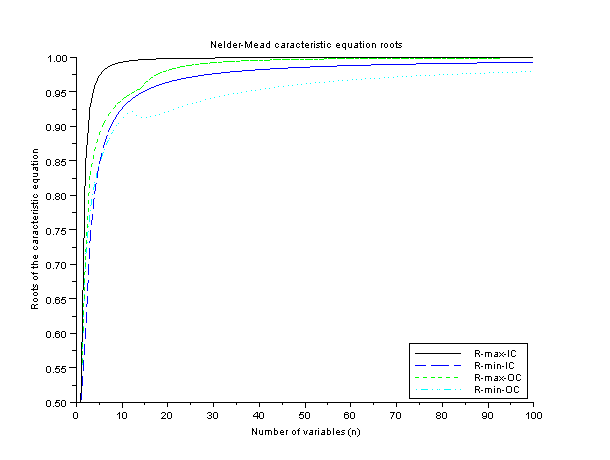
\includegraphics[width=10cm]{neldermead-roots.png}
\end{center}
\caption{Modulus of the roots of the characteristic equations of the Nelder-Mead method with standard 
coefficients -- R-max-IC is the maximum of the modulus of the root of the Inside Contraction steps}
\label{fig-nm-roots}
\end{figure}

\subsection{With variable parameters}

In this section, we analyze the roots of the characteristic 
equation with \emph{variable} inside and outside contraction
coefficients.

\emph{Outside contraction} \\
If the outside contraction step is repeatedly performed
with variable $\mu_{oc} \in }0,\mu_r[$, then 
\begin{eqnarray}
\bv^{(k+n)} &=& \overline{\bold{v}}^{(k)} 
+ \mu_{oc} \left( \overline{\bold{v}}^{(k)} - \bv^{(k)}\right) \\
&=& (1 + \mu_{oc} ) \overline{\bold{v}}^{(k)} - \mu_{oc} \bv^{(k)}
\end{eqnarray}
By plugging the definition of the centroid into the previous equality, we 
find the recurrence formula
\begin{eqnarray}
n \bv^{(k+n)} - (1 + \mu_{oc} ) \bv^{(k+1)} - \ldots - (1 + \mu_{oc} ) \bv^{(k+n-1)} + n\mu_{oc}\bv^{(k)} = 0
\end{eqnarray}

The associated characteristic equation is 
\begin{eqnarray}
\label{recurrence-variable}
n \mu^n - (1 + \mu_{oc} ) \mu^{n-1} - \ldots - (1 + \mu_{oc} ) \mu + n \mu_{oc} = 0.
\end{eqnarray}

\emph{Inside contraction} \\
We suppose that the inside contraction step is repeatedly performed
with $-1 < \mu_{ic} < 0$. The characteristic equation is the same as \ref{recurrence-variable},
but it is here studied in the range $\mu_{ic}\in]-1, 0[$.

To study the convergence of the method, we simply have 
to study the roots of equation \ref{recurrence-variable}, where 
the range $]-1,0[$ corresponds to the inside contraction (with $-1/2$ 
as the standard value) and where the range $]0,\mu_r[$ corresponds to the outside contraction (with $1/2$ 
as the standard value).

In the following Scilab script, we compute the minimum and 
maximum root of the characteristic equation, with $n$ fixed.

\lstset{language=scilabscript}
\begin{lstlisting}
//
// rootsvariable --
//   Compute roots of the characteristic equation 
//   of Nelder-Mead with variable coefficient mu.
// Polynomial for outside/inside contraction :
// n mu - (1+mu)x - ... - (1+mu)x^(n-1) + n x^(n) = 0
//
function [rmin , rmax] = rootsvariable ( n , mu )
  coeffs = zeros(1,n+1);
  coeffs(1) = n * mu
  coeffs(2:n) = -(1+mu)
  coeffs(n+1) = n
  p=poly(coeffs,"x","coeff")
  r = roots(p , "e")
  rmin = min(abs(r))
  rmax = max(abs(r))
  mprintf("%f & %f & %f\\\\\n", mu, rmin, rmax)
endfunction

function drawfigure_variable ( n , nmumax )
  rmintable = zeros(1,nmumax)
  rmaxtable = zeros(1,nmumax)
  mutable = linspace ( -1 , 1 , nmumax ) 
  for index = 1 : nmumax
    mu = mutable ( index )
    [rmin , rmax ] = rootsvariable ( n , mu )
    rmintable ( index ) = rmin
    rmaxtable ( index ) = rmax
  end
  plot2d ( mutable , [ rmintable' , rmaxtable' ] )
  f = gcf();
  pause
  f.children.title.text = "Nelder-Mead characteristic equation roots";
  f.children.x_label.text = "Contraction coefficient";
  f.children.y_label.text = "Roots of the characteristic equation";
  captions(f.children.children.children,["R-max","R-min"]);
  f.children.children(1).legend_location="in_lower_right";
  for i = 1:2
  mypoly = f.children.children(2).children(i);
  mypoly.foreground=i;
  mypoly.line_style=i;
  end
  xs2png(0,"neldermead-roots-variable.png");
endfunction

\end{lstlisting}

The figure \ref{fig-nm-roots-variable} presents the minimum
and maximum modulus of the roots of the characteristic equation
with $n=10$. The result is that when $\mu_{oc}$ is close to 0, the 
minimum root has a modulus close to 0. The maximum root remains close to 
1, whatever the value of the contraction coefficient.
This result would mean that either modifying the contraction
coefficient has no effect (because the maximum modulus of the roots 
is close to 1) or diminishing the contraction coefficient should 
improve the convergence speed (because the minimum modulus of the 
roots gets closer to 0). This is the expected result because
the more the contraction coefficient is close to 0, the more the new 
vertex is close to 0, which is, in our particular situation, the 
global minimizer. No general conclusion can be drawn from this single 
experiment.

\begin{figure}
\begin{center}
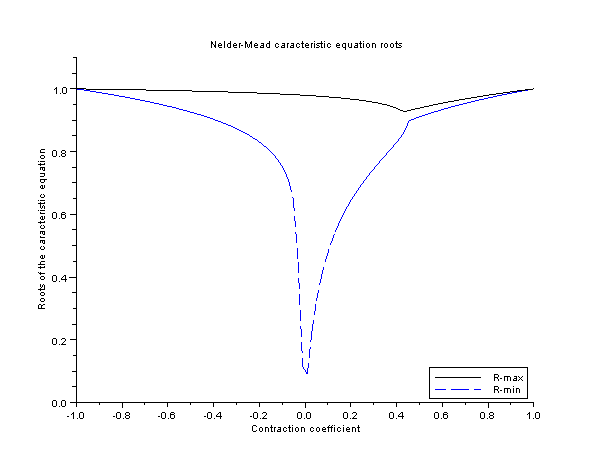
\includegraphics[width=10cm]{neldermead-roots-variable.png}
\end{center}
\caption{Modulus of the roots of the characteristic equations of the Nelder-Mead method with variable 
contraction coefficient and $n=10$ -- R-max is the maximum of the modulus of the root of the 
characteristic equation}
\label{fig-nm-roots-variable}
\end{figure}

\section{Numerical experiments}

In this section, we present some numerical experiments 
with the Nelder-Mead algorithm.
The two first numerical experiments involve simple quadratic functions.
These experiments allows to see the difference between
Spendley's et al. algorithm and the Nelder-Mead algorithm.
We then present several experiments taken from the bibliography.
The O'Neill experiments \cite{O'Neill1971AAF} are performed in order 
to check that our algorithm is a correct implementation.
We then present several numerical experiments where the Nelder-Mead
does not converge properly.
We analyze the Mc Kinnon counter example 
from \cite{589109}. We show the behavior of the 
Nelder-Mead simplex method for a family of examples which cause the 
method to converge to a non stationnary point.
We analyze the counter examples presented by Han in his Phd thesis \cite{Han2000}.
In these experiments, the Nelder-Mead algorithm degenerates by applying repeatedly
the inside contraction step.
We also reproduce numerical experiments extracted from Torczon's Phd Thesis 
\cite{Torczon89multi-directionalsearch}, where Virginia Torczon 
presents the multi-directional direct search algorithm. 

\subsection{Quadratic function}

The function we try to minimize is the following quadratic 
in 2 dimensions 

\begin{eqnarray}
f(x_1,x_2) = x_1^2 + x_2^2 - x_1 x_2
\end{eqnarray}

The stopping criteria is based on the relative size of the simplex 
with respect to the size of the initial simplex 

\begin{eqnarray}
\sigma(S) < tol \times \sigma(S_0)
\end{eqnarray}

The initial simplex is computed from the coordinate axis and the unit length.
The numerical results are presented in table \ref{fig-nm-numexp1-table}.

\begin{figure}[htbp]
\begin{center}
%\begin{tiny}
\begin{tabular}{|l|l|}
\hline
Iterations & 65 \\
Function Evaluations & 127 \\
$x_0$ & $(2.0,2.0)$ \\
Relative tolerance on simplex size & $10^{-8}$ \\
Exact $x^\star$ & $(0.,0.)$\\
Computed $x^\star$ & $(7.3e-10 , -2.5e-9)$\\
Computed $f(x^\star)$ & $8.7e-18$\\
\hline
\end{tabular}
%\end{tiny}
\end{center}
\caption{Numerical experiment with Nelder-Mead method on the quadratic function
$f(x_1,x_2) = x_1^2 + x_2^2 - x_1 x_2$}
\label{fig-nm-numexp1-table}
\end{figure}


The various simplices generated during the iterations are 
presented in figure \ref{fig-nm-numexp1-historysimplex}.
The method use reflections in the early iterations. Then there
is no possible improvement using reflections and shrinking is necessary.

\begin{figure}
\begin{center}
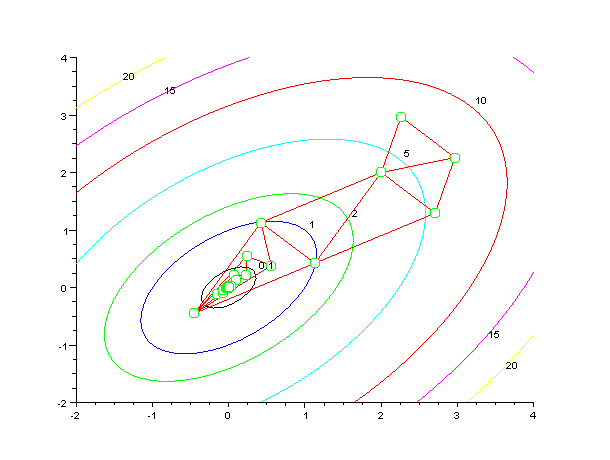
\includegraphics[width=10cm]{quad2bis-nm-simplexcontours.png}
\end{center}
\caption{Nelder-Mead numerical experiment -- history of simplex}
\label{fig-nm-numexp1-historysimplex}
\end{figure}

The figure \ref{fig-nm-numexp1-sigma} presents the history of the oriented
length of the simplex. The length is updated at each iteration, which 
generates a continuous evolution of the length, compared to the 
step-by-step evolution of the simplex with the Spendley et al. algorithm.

\begin{figure}
\begin{center}
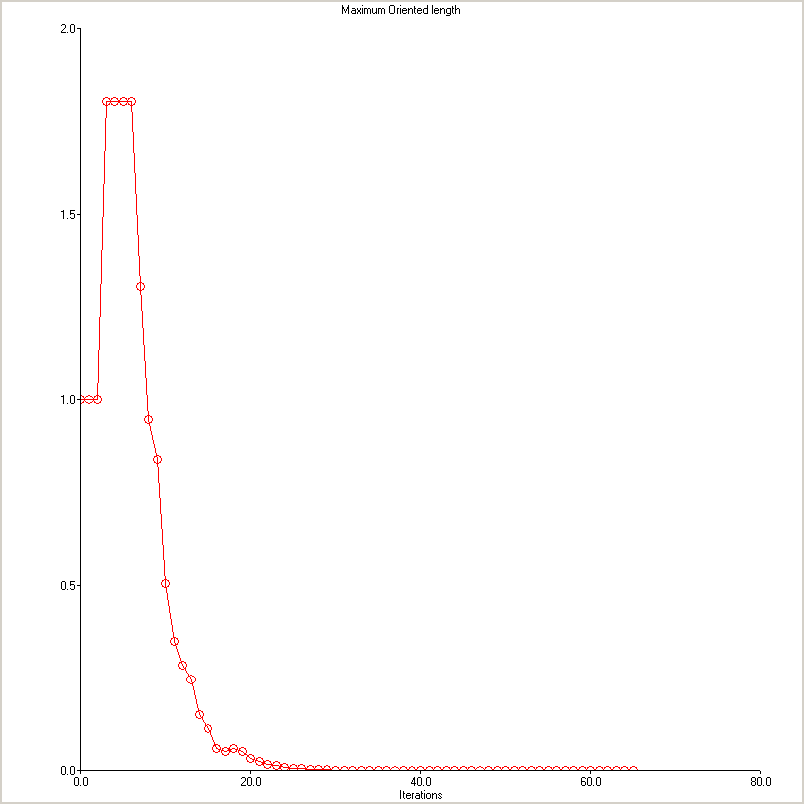
\includegraphics[width=10cm]{quad2bis-nm-history-sigma.png}
\end{center}
\caption{Nelder-Mead numerical experiment -- history of length of simplex}
\label{fig-nm-numexp1-sigma}
\end{figure}

The convergence is quite fast in this case, since less than 60 iterations
allow to get a function value lower than $10^{-15}$, as shown in 
figure \ref{fig-nm-numexp1-logfopt}.

\begin{figure}
\begin{center}
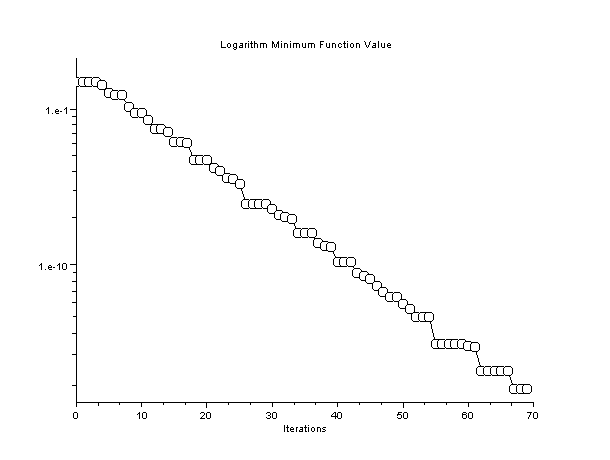
\includegraphics[width=10cm]{quad2bis-nm-history-logfopt.png}
\end{center}
\caption{Nelder-Mead numerical experiment -- history of logarithm of function}
\label{fig-nm-numexp1-logfopt}
\end{figure}

\subsubsection{Badly scaled quadratic function}

The function we try to minimize is the following quadratic 
in 2 dimensions 
\begin{eqnarray}
\label{quadratic-nm-function2}
f(x_1,x_2) = a x_1^2 + x_2^2,
\end{eqnarray}
where $a>0$ is a chosen scaling parameter. 
The more $a$ is large, the more difficult the problem is 
to solve with the simplex algorithm.

We set the maximum number of function evaluations to 400.
The initial simplex is computed from the coordinate axis and the unit length.

The numerical results are presented in table \ref{fig-nm-numexp2-table},
where the experiment is presented for $a=100$. We can check that the 
number of function evaluation (161 function evaluations) is much lower than the number 
for the fixed shape Spendley et al. method (400 function evaluations)
and that the function value at optimum is very accurate ($f(x^\star)\approx 1.e-17$
compared to Spendley's et al. $f(x^\star) \approx 0.08$).

\begin{figure}[h]
\begin{center}
%\begin{tiny}
\begin{tabular}{|l|l|l|}
\hline
& Nelder-Mead & Spendley et al.\\
\hline
Iterations & 83  & 340 \\
Function Evaluations & 161 & 400 \\
$a$ & $100.0$ & - \\
$x_0$ & $(10.0,10.0)$ & - \\
Relative tolerance on simplex size & - \\
Exact $x^\star$ & $(0.,0.)$ & -\\
Computed $x^\star$ & $(2.e-10, -3.e-9)$& $(0.001,0.2)$\\
Computed $f(x^\star)$ & $1.e-17$ & $0.08$\\
\hline
\end{tabular}
%\end{tiny}
\end{center}
\caption{Numerical experiment with Nelder-Mead method on a badly scaled quadratic function.
The variable shape Nelder-Mead algorithm improves the accuracy of the result compared
to the fixed shaped Spendley et al. method.}
\label{fig-nm-numexp2-table}
\end{figure}

In figure \ref{fig-nm-numexp2-scaling}, we analyze the 
behavior of the method with respect to scaling.
We check that the method behave very smoothly, with a very 
small number of additional function evaluations when the 
scaling deteriorates. This shows how much the Nelder-Mead algorithms 
improves over Spendley's et al. method.

\begin{figure}[htbp]
\begin{center}
%\begin{tiny}
\begin{tabular}{|l|l|l|l|}
\hline
$a$ & Function evaluations & Computed $f(x^\star)$ & Computed $x^\star$\\
$1.0$ & 139 & $8.0e-18$ & $(2.e-9 -1.e-9)$\\
$10.0$ & 151 & $7.0e-17$ & $(5.e-10 2.e-9)$\\
$100.0$ & 161 & $1.0e-17$ & $(2.e-10 -3.e-9)$ \\
$1000.0$ & 165 & $1.0e-17$ & $(-1.e-010 9.e-10)$\\
$10000.0$ & 167 & $3.0e-17$ & $(5.0e-11,-1.0e-10)$ \\
\hline
\end{tabular}
%\end{tiny}
\end{center}
\caption{Numerical experiment with Spendley's et al. method on a badly scaled quadratic function}
\label{fig-nm-numexp2-scaling}
\end{figure}

\subsection{Sensitivity to dimension}

In this section, we try to reproduce the result 
presented by Han and Neumann \cite{HanNeumann2006}, which shows that the 
convergence rate of the Nelder-Mead algorithms rapidly 
deteriorates when the number of variables increases.
The function we try to minimize is the following quadratic 
in n-dimensions 
\begin{eqnarray}
\label{quadratic-function3}
f(\bold{x}) = \sum_{i=1,n} x_i^2.
\end{eqnarray}

The initial simplex is computed from the coordinate axis and the unit length.
The initial guess is at 0 so that the first vertex is the origin ; 
this vertex is never updated during the iterations.

The figure \ref{fig-nm-numexp3-dimension} presents the results of this 
experiment for $n=1,19$. 

During the iterations, no shrink steps are performed. The 
algorithm performs reflections, inside and outside contractions.
The figure \ref{fig-nm-numexp3-steps} shows the detailed sequence of 
iterations for $n=10$. We see that there is no general 
pattern for the iterations. One can check, however, that there 
are never no more than $n$ consecutive reflection steps, which is 
as expected. After one or more contractions, the reflection
steps move the worst vertices toward better function values.
But there are only $n+1$ vertices so that the $n$ worst 
vertices are moved in at most $n$ reflection steps.

\begin{figure}[htbp]
\begin{center}
%\begin{tiny}
\begin{verbatim}
I I I I I I I I I I I I I I I I I I I I R R R R R R R R R R R R R I O 
R R R R R R R R R R R R R I R I I R I R O I I I I R I R I I R O I R R 
R R I R I R I R R R R R R R I R R R R I R I I R I R I I I R R I I I R 
R R I R R I R R R R R R I R I R R R R R I R R O R R I O I O R R R R I 
I I O R I R R R R R R I I I R R I I R R R O R I I R R R I R I I O I R 
I R R O I I R R R R I R R O I R R O R I R I R I R R I R I R R R I I I 
I I O R R R R I I I R R R I I I R R R I I I I R R R R I I R R R R I R 
R R I O I R R I I R R R R O I R I I R R R R R R O R R R O I R R I I I 
I O R I I I R I I I I R R I I R R I R R R R R R I R R I I R R O R I I 
O R I R O O R O I I R I I I R I I R R R R R R R R R R R R I R R O I R 
I O I R I I I I R I I R I I R I R O R I O R I R I R R R O R I R R R I 
I R I R R R I R I R R R R I I R R I R R R R I I R R R R I I R I R I I 
O I R I I R R R R R R R R I O I R R I I I R I R I I I I R R R R I R R 
I R I R R R R I I R R R I I I I R I I I I R I R R I R I O R R R I R I 
O I R R I I R R I R R R R O R R R R I O R R R I R I I I I R I R R R R 
R I I R I I R R R R R O R R R I R R R R I R I R R I R I I R R I I R R 
I I I I R R R R R R R R R I R R O R R R R R O I I I I R I I R O I I R 
R R R R I I I R R
\end{verbatim}
%\end{tiny}
\end{center}
\caption{Numerical experiment with Nelder-Mead method on a generalized 
quadratic function - steps of the algorithm : I = inside contraction, O = outside contraction, 
R = reflection, S = shrink}
\label{fig-nm-numexp3-steps}
\end{figure}

The figure \ref{fig-nm-numexp3-nbsteps} presents the number and 
the kind of steps performed during the iterations for $n=1,19$.
It appears that the number of shrink steps and expansion steps is zero, as expected.
More interesting is that the number of reflection is 
larger than the number of inside contraction when $n$ 
is large. The number of outside contraction is always 
the smallest in this case.

\begin{figure}[htbp]
\begin{center}
%\begin{tiny}
\begin{tabular}{|l|l|l|l|l|l|}
\hline
$n$ & \# Reflections & \# Expansion & \# Inside & \# Outside & \#Shrink\\
 & & & Contractions & Contractions & \\
\hline
1 & 0 & 0 & 27 & 0 & 0\\
2 & 0 & 0 & 5 & 49 & 0\\
3 & 54 & 0 & 45 & 36 & 0\\
4 & 93 & 0 & 74 & 34 & 0\\
5 & 123 & 0 & 101 & 33 & 0\\
6 & 170 & 0 & 122 & 41 & 0\\
7 & 202 & 0 & 155 & 35 & 0\\
8 & 240 & 0 & 178 & 41 & 0\\
9 & 267 & 0 & 205 & 40 & 0\\
10 & 332 & 0 & 234 & 38 & 0\\
11 & 381 & 0 & 267 & 36 & 0\\
12 & 476 & 0 & 299 & 32 & 0\\
13 & 473 & 0 & 316 & 42 & 0\\
14 & 545 & 0 & 332 & 55 & 0\\
15 & 577 & 0 & 372 & 41 & 0\\
16 & 635 & 0 & 396 & 46 & 0\\
17 & 683 & 0 & 419 & 52 & 0\\
18 & 756 & 0 & 445 & 55 & 0\\
19 & 767 & 0 & 480 & 48 & 0\\
\hline
\end{tabular}
%\end{tiny}
\end{center}
\caption{Numerical experiment with Nelder-Mead method on a generalized quadratic function -- number 
and kinds of steps performed}
\label{fig-nm-numexp3-nbsteps}
\end{figure}

We check that the number of function evaluations 
increases approximately linearly with the dimension of the problem in
figure \ref{fig-nm-numexp3-fvn}. A rough rule of thumb is that, for $n=1,19$, 
the number of function evaluations is equal to $100n$.

\begin{figure}[htbp]
\begin{center}
%\begin{tiny}
\begin{tabular}{|l|l|l|l|}
\hline
$n$ & Function evaluations & Iterations & $\rho(S_0,n)$\\
\hline
1 & 56 & 28 & 0.5125321059829373\\
2 & 111 & 55 & 0.71491052830553248\\
3 & 220 & 136 & 0.87286283470760984\\
4 & 314 & 202 & 0.91247307800713973\\
5 & 397 & 258 & 0.93107793607270162\\
6 & 503 & 334 & 0.94628781077508028\\
7 & 590 & 393 & 0.95404424343636474\\
8 & 687 & 460 & 0.96063768057900478\\
9 & 767 & 513 & 0.96471820169933631\\
10 & 887 & 605 & 0.97000569588245511\\
11 & 999 & 685 & 0.97343652480535203\\
12 & 1151 & 808 & 0.97745310525741003\\
13 & 1203 & 832 & 0.97803465666405531\\
14 & 1334 & 933 & 0.98042500139065414\\
15 & 1419 & 991 & 0.98154526298964495\\
16 & 1536 & 1078 & 0.98305435726547608\\
17 & 1643 & 1155 & 0.98416149958157839\\
18 & 1775 & 1257 & 0.98544909490809807\\
19 & 1843 & 1296 & 0.98584701106083183\\
\hline
\end{tabular}
%\end{tiny}
\end{center}
\caption{Numerical experiment with Nelder-Mead method on a generalized quadratic function}
\label{fig-nm-numexp3-dimension}
\end{figure}

\begin{figure}
\begin{center}
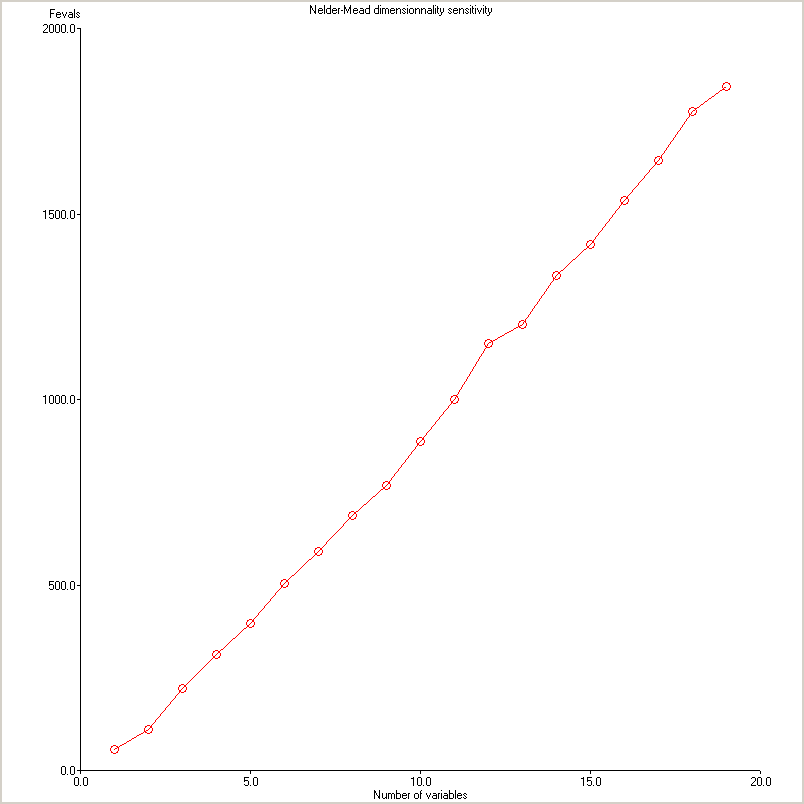
\includegraphics[width=10cm]{neldermead-dimension-nfevals.png}
\end{center}
\caption{Nelder-Mead numerical experiment -- number of function evaluations 
depending on the number of variables}
\label{fig-nm-numexp3-fvn}
\end{figure}

The figure \ref{fig-nm-numexp3-rho} presents the rate of convergence 
depending on the number of variables. The figure shows that 
the rate of convergence rapidly gets close to 1 when the number 
of variables increases. That shows that the rate of convergence 
is slower and slower as the number of variables increases, as 
explained by Han \& Neumann.

\begin{figure}
\begin{center}
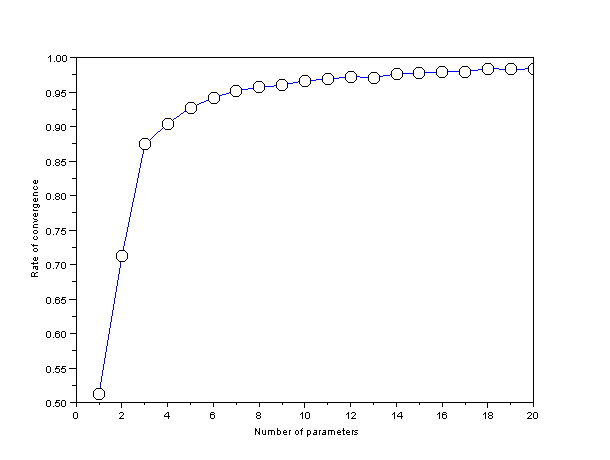
\includegraphics[width=10cm]{neldermead-dimension-rho.png}
\end{center}
\caption{Nelder-Mead numerical experiment -- rate of convergence 
depending on the number of variables}
\label{fig-nm-numexp3-rho}
\end{figure}

\subsection{O'Neill test cases}

In this section, we present the results by O'Neill, who 
implemented a fortran 77 version of the Nelder-Mead algorithm
\cite{O'Neill1971AAF}.

The O'Neill implementation of the Nelder-Mead algorithm has the following 
particularities 
\begin{itemize}
\item the initial simplex is computed from the axes and a (single) length,
\item the stopping rule is based on variance (not standard deviation) of function value,
\item the expansion is greedy, i.e. the expansion point is accepted if it is better than the lower point,
\item an automatic restart is performed if a factorial test shows that the 
computed optimum is greater than a local point computed with a relative 
epsilon equal to 1.e-3.
\end{itemize}

The following tests are presented by O'Neill :

\begin{itemize}
\item Rosenbrock's parabolic valley \cite{citeulike:1903787}
\begin{eqnarray}
\label{nm-oneill-rosenbrock}
f(x_1,x_2) = 100(x_2 - x_1^2)^2 + (1-x_1)^2
\end{eqnarray}
with starting point $(x_1,x_2) = (-1.2,1.0)$
\item Powell's quartic function \cite{Powell08011962}
\begin{eqnarray}
\label{nm-oneill-powell}
f(x_1,x_2,x_3,x_4) = (x_1 + 10x_2)^2 + 5 ( x_3 - x_4)^2 + (x_2 - 2x_3)^4 + 10 (x_1 - x_4)^4
\end{eqnarray}
with starting point $(x_1,x_2,x_3,x_4) = (3,-1,0,1)$
\item Fletcher and Powell's helical valley \cite{R.Fletcher08011963}
\begin{eqnarray}
\label{nm-oneill-fletcherpowell}
f(x_1,x_2,x_3) = 100\left(x_3 + 10\theta(x_1,x_2)\right)^2 
+ \left(\sqrt{x_1^2 + x_2^2} - 1\right)^2  + x_3^2
\end{eqnarray}
where 
\begin{eqnarray}
\label{nm-oneill-fletcherpowelltheta}
2\pi \theta(x_1,x_2) &=& \arctan(x_2,x_1), x_1>0\\
&=& \pi + \arctan(x_2,x_1), x_1<0\\
\end{eqnarray}
with starting point $(x_1,x_2,x_3) = (-1,0,0)$. Note
that since $\arctan(0/0)$ is not defined neither 
the function $f$ on the line $(0,0,x_3)$. This line is excluded 
by assigning a very large value to the function.
\item the sum of powers 
\begin{eqnarray}
\label{nm-oneill-powers}
f(x_1,\ldots,x_{10}) = \sum_{i=1,10} x_i^4
\end{eqnarray}
with starting point $(x_1,\ldots,x_{10}) = (1,\ldots,1)$
\end{itemize}

The parameters are set to 

\begin{itemize}
\item $REQMIN=10^{-16}$, the absolute tolerance on the variance of the function 
values in the simplex,
\item $STEP = 1.0$, the absolute side length of the initial simplex,
\item $ICOUNT$, the maximum number of function evaluations.
\end{itemize}

The table \ref{fig-nm-oneill-table} presents the results which were 
computed by O'Neill compared with our software.
For most experiments, the results are very close in terms of 
number of function evaluations. 
The problem \#4 exhibits a completely different behavior than the 
results presented by O'Neill. For us, the maximum number of function evaluations
is reached (i.e. 1000 function evaluations), whereas for O'Neill, the algorithm 
is restarted and gives the result with 474 function evaluations. 
We did not find any explanation for this behavior. A possible cause of 
difference may be the floating point system which are different and may 
generate different simplices in the algorithms.
Although the CPU times cannot be 
compared (the article is dated 1972 !), let's mention 
that the numerical experiment were performed by O'Neill
on a ICL 4-50 where the two problem 1 and 2 were solved in 3.34 seconds
and the problems 3 and 4 were solved in 22.25 seconds.


\begin{figure}[htbp]
\begin{center}
%\begin{tiny}
\begin{tabular}{|l|l|l|l|l|l|l|}
\hline
Author & Problem & Function & No. of Restarts & Function Value & Iterations & CPU\\
& & Evaluations & & & & Time \\
\hline
O'Neill & 1 & 148 & 0 & 3.19 e-9 & ? & ? \\
Baudin & 1 & 149 & 0 & 1.15 e-7 & 79 & 0.238579 \\
\hline
O'Neill & 2 & 209 & 0 & 7.35 e-8 & ? & ?  \\
Baudin & 2 & 224 & 0 & 1.07 e-8 & 126 & 0.447958 \\
\hline
O'Neill & 3 & 250 & 0 & 5.29 e-9 & ? & ? \\
Baudin & 3 & 255 & 0 & 4.56 e-8 & 137 & 0.627493 \\
\hline
O'Neill & 4 & 474 & 1 & 3.80 e-7 & ? & ? \\
Baudin & 4 & 999 & 0 & 5.91 e-9 & 676 & - \\
\hline
\end{tabular}
%\end{tiny}
\end{center}
\caption{Numerical experiment with Nelder-Mead method on O'Neill test cases - O'Neill results and our results}
\label{fig-nm-oneill-table}
\end{figure}

\subsection{Convergence to a non stationnary point}
\label{section-mcKinnon}

In this section, we analyze the Mc Kinnon counter example 
from \cite{589109}. We show the behavior of the 
Nelder-Mead simplex method for a family of examples which cause the 
method to converge to a non stationnary point.

Consider a simplex in two dimensions with vertices at 0 (i.e. the origin),
$\bv^{(n+1)}$ and $\bv^{(n)}$. Assume that 

\begin{eqnarray}
\label{mckinnon-sortedfv}
f(0) < f(\bv^{(n+1)}) < f(\bv^{(n)}).
\end{eqnarray}

The centroid of the simplex is $\overline{\bv} = \bv^{(n+1)}/2$, the midpoint
of the line joining the best and second vertex. The reflected 
point is then computed as 

\begin{eqnarray}
\label{mckinnon-reflection}
\br^{(n)} = \overline{\bv} + \rho ( \overline{\bv} - \bv^{(n)} ) 
= \bv^{(n+1)} - \bv^{(n)}
\end{eqnarray}

Assume that the reflection point $\br^{(n)}$ is rejected, i.e. that 
$f(\bv^{(n)}) < f(\br^{(n)})$. In this case, the inside contraction 
step is taken and the point $\bv^{(n+2)}$ is computed using the 
reflection factor $-\gamma = -1/2$ so that 

\begin{eqnarray}
\label{mckinnon-insidecontraction}
\bv^{(n+2)} = \overline{\bv} - 
\gamma ( \overline{\bv} - \bv^{(n)} ) 
= \frac{1}{4} \bv^{(n+1)} - \frac{1}{2} \bv^{(n)}
\end{eqnarray}

Assume then that the inside contraction point is accepted, i.e. $f(\bv^{(n+2)}) < f(\bv^{(n+1)})$.
If this sequence of steps repeats, the simplices are subject to the 
following linear recurrence formula

\begin{eqnarray}
\label{mckinnon-reccurence}
4 \bv^{(n+2)} - \bv^{(n+1)} + 2 \bv^{(n)} = 0
\end{eqnarray}

Their general solutions are of the form 

\begin{eqnarray}
\bv^{(n)} = \lambda_1^k a_1 + \lambda_2^k a_2
\end{eqnarray}
where ${\lambda_i}_{i=1,2}$ are the roots of the characteristic equation and 
${a_i}_{i=1,2} \in \RR^n$. 
The characteristic equation is 
\begin{eqnarray}
\label{mckinnon-caracequation}
4 \lambda^2 - \lambda + 2 \lambda = 0
\end{eqnarray}
and has the roots 
\begin{eqnarray}
\label{mckinnon-roots}
\lambda_1 = \frac{1 + \sqrt{33}}{8}\approx 0.84307, 
\qquad \lambda_2 = \frac{1 - \sqrt{33}}{8} \approx -0.59307
\end{eqnarray}

After Mc Kinnon has presented the computation of the roots of the 
characteristic equation, he presents a special initial simplex 
for which the simplices degenerates because of repeated failure by inside 
contraction (RFIC in his article). Consider the initial simplex with
vertices $\bv^{(0)} = (1,1)$ and $\bv^{(1)} = (\lambda_1,\lambda_2)$ and 
$0$. If follows that the particular solution for these initial 
conditions is $\bv^{(n)} = (\lambda_1^n,\lambda_2^n)$.

Consider the function $f(x_1,x_2)$ given by 
\begin{eqnarray}
\label{mckinnon-function}
f(x_1,x_2) &=& \theta \phi |x_1|^\tau + x_2 + x_2^2, \qquad x_1\leq 0,\\
&=&\theta x_1^\tau + x_2 + x_2^2, \qquad x_1\geq 0.
\end{eqnarray}
where $\theta$ and $\phi$ are positive constants. Note that $(0,-1)$
is a descent direction from the origin $(0,0)$ and that f is stricly convex 
provided $\tau>1$. $f$ has continuous first derivatives if $\tau>1$, continuous second 
derivatives if $\tau>2$ and continuous third derivatives if $\tau>3$.

Mc Kinnon computed the conditions on $\theta,\phi$ and $\tau$
so that the function values are ordered as expected, i.e. so that the 
reflection step is rejected and the inside contraction is accepted.
Examples of values which makes these equations hold are as follows :
for $\tau=1$, $\theta=15$ and $\phi = 10$, 
for $\tau=2$, $\theta=6$ and $\phi = 60$ and
for $\tau=3$, $\theta=6$ and $\phi = 400$.

We consider here the more regular case $\tau=3$, $\theta=6$
and $\phi = 400$, i.e. the function is defined by 
\begin{eqnarray}
\label{mckinnon-function3}
f(x_1,x_2) &=& - 2400 x_1^3 + x_2 + x_2^2, \qquad x_1\leq 0, \\
&=& 6 x_1^3 + x_2 + x_2^2, \qquad x_1\geq 0.
\end{eqnarray}

The figure \ref{fig-nm-numexp-mckinnon} shows the contour plot of this function and the first 
steps of the Nelder-Mead method.
The global minimum is located at $(0,-1/2)$.
Notice that the simplex degenerates to the
point $(0,0)$, which is a non stationnary point.

\begin{figure}
\begin{center}
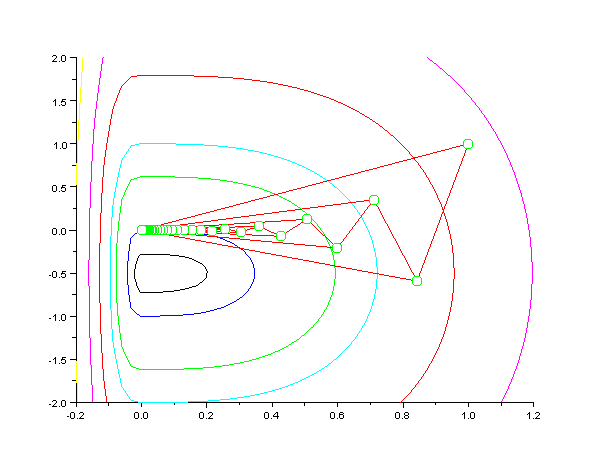
\includegraphics[width=10cm]{mckinnon-history-simplex.png}
\end{center}
\caption{Nelder-Mead numerical experiment -- Mc Kinnon example for convergence toward
a non stationnary point}
\label{fig-nm-numexp-mckinnon}
\end{figure}

The figure \ref{fig-nm-numexp-mckinnon-detail} presents the first steps 
of the algorithm in this numerical experiment. Because of the 
particular shape of the contours of the function, the reflected 
point is always worse that the worst vertex $\bx_{n+1}$. This 
leads to the inside contraction step. The vertices constructed 
by Mc Kinnon are so that the situation loops without end.

\begin{figure}
\begin{center}
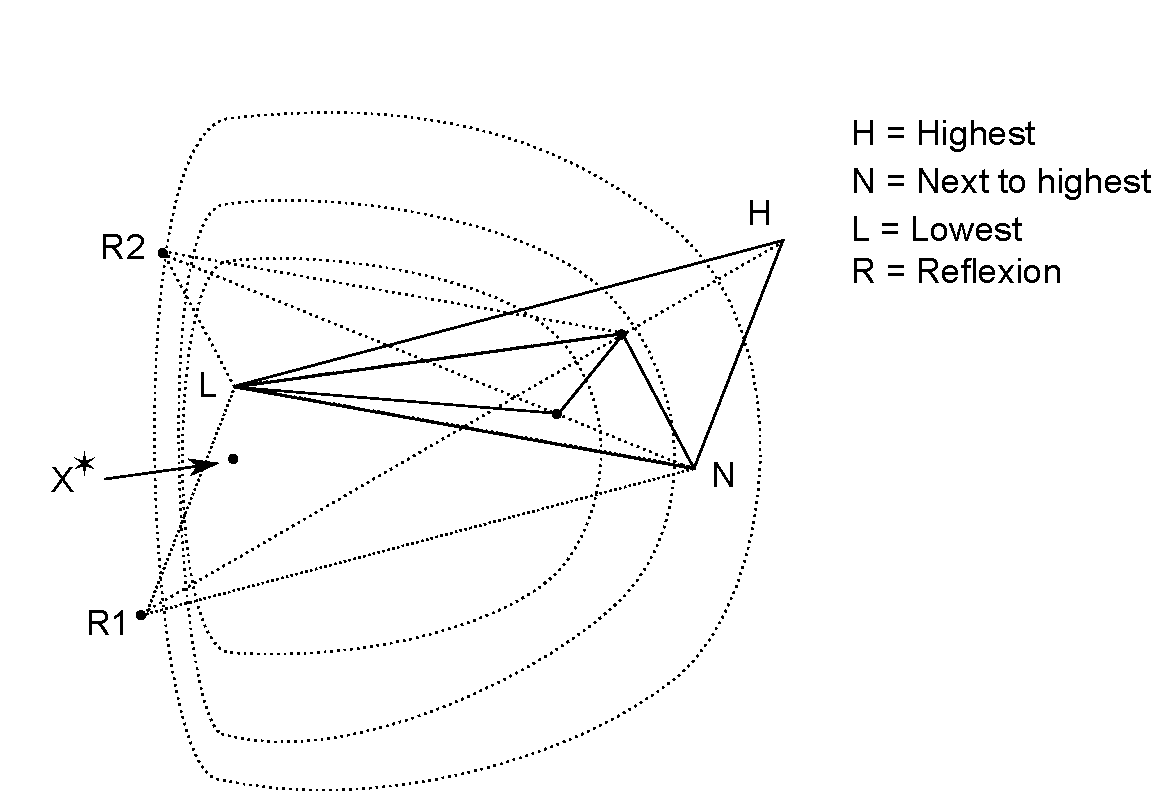
\includegraphics[width=10cm]{mcKinnon-insidecontraction.pdf}
\end{center}
\caption{Nelder-Mead numerical experiment -- Detail of the first steps.
The simplex converges to a non stationnary point, after repeated 
inside contractions.}
\label{fig-nm-numexp-mckinnon-detail}
\end{figure}

\subsection{Han counter examples}

In his Phd thesis \cite{Han2000}, Han presents two counter examples
in which the Nelder-Mead algorithm degenerates by applying repeatedly
the inside contraction step.

\subsubsection{First counter example}

The first counter example is based on the function 
\begin{eqnarray}
\label{han-function1}
f(x_1,x_2) &=& x_1^2 + x_2 ( x_2 + 2 ) ( x_2 - 0.5 ) ( x_2 - 2 )
\end{eqnarray}

This function is nonconvex, bounded below and has bounded level 
sets. The initial simplex is chosen as $S_0 = [(0.,-1),(0,1),(1,0)]$.
Han proves that the Nelder-Mead algorithm generates a sequence of simplices
$S_k = [(0.,-1),(0,1),(\frac{1}{2^k},0)]$.

The figure \ref{fig-nm-numexp-han1} presents the isovalues and the 
simplices during the steps of the Nelder-Mead algorithm.
Note that the limit simplex contains no minimizer of the function.
The failure is caused by repeated inside contractions.

\begin{figure}
\begin{center}
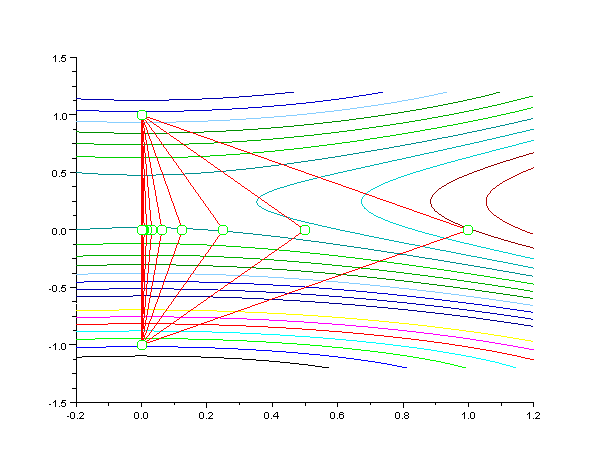
\includegraphics[width=10cm]{han1-history-simplex.png}
\end{center}
\caption{Nelder-Mead numerical experiment -- Han example \#1 for convergence toward
a non stationnary point}
\label{fig-nm-numexp-han1}
\end{figure}

\subsubsection{Second counter example}

The second counter example is based on the function 
\begin{eqnarray}
\label{han-function2}
f(x_1,x_2) &=& x_1^2 + \rho(x_2)
\end{eqnarray}
where $\rho$ is a continuous convex function with bounded level
sets defined by
\begin{eqnarray}
\label{han-function2-rho}
\left\{
\begin{array}{ll}
\rho(x_2) =0, &\qquad \textrm{if} \qquad |x_2|\leq 1, \\
\rho(x_2)\geq 0, &\qquad \textrm{if} \qquad |x_2|> 1.
\end{array}
\right.
\end{eqnarray}
The example given by Han for such a $\rho$ function is 
\begin{eqnarray}
\label{han-function2-rho2}
\rho(x_2) =
\left\{
\begin{array}{ll}
0, &\qquad \textrm{if} \qquad |x_2|\leq 1, \\
x_2 - 1, &\qquad \textrm{if} \qquad x_2> 1, \\
-x_2 - 1, &\qquad \textrm{if} \qquad x_2 < -1.
\end{array}
\right.
\end{eqnarray}

The initial simplex is chosen as $S_0 = [(0.,1/2),(0,-1/2),(1,0)]$.
Han prooves that the Nelder-Mead algorithm generates a sequence of simplices
$S_k = [(0.,1/2),(0,-1/2),(\frac{1}{2^k},0)]$.

The figure \ref{fig-nm-numexp-han2} presents the isovalues and the 
simplices during the steps of the Nelder-Mead algorithm.
The failure is caused by repeated inside contractions.

\begin{figure}
\begin{center}
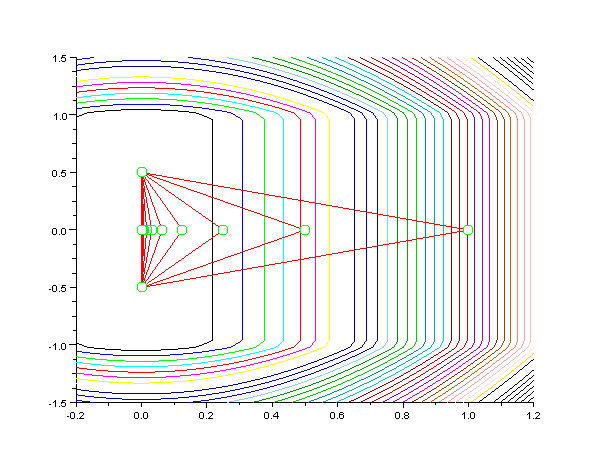
\includegraphics[width=10cm]{han2-history-simplex.png}
\end{center}
\caption{Nelder-Mead numerical experiment -- Han example \#2 for convergence toward
a non stationnary point}
\label{fig-nm-numexp-han2}
\end{figure}

These two examples of non convergence show that the Nelder-Mead method may unreliable.
They also reveal that the Nelder-Mead method can generate simplices which collapse 
into a degenerate simplex, by applying repeated inside contractions.

\subsection{Torczon's numerical experiments}

In her Phd Thesis \cite{Torczon89multi-directionalsearch}, Virginia Torczon 
presents the multi-directional direct search algorithm. In order to analyze the 
performances of her new algorithm, she presents some interesting numerical 
experiments with the Nelder-Mead algorithm. 
These numerical experiments are based on the collection of test problems \cite{355943},
published in the ACM by Mor\'e, Garbow and Hillstrom in 1981. 
These test problems are associated with varying number of variables.
In her Phd, Torczon presents numerical experiments with $n$ from 8 
to 40.
The stopping rule is based on the relative size of the simplex. 
The angle between the descent direction (given by the worst point and the centroid), and the
gradient of the function is computed when the algorithm is stopped.
Torczon shows that, when the tolerance on the relative simplex size is decreased, the 
angle converges toward 90 \degre. This fact is observed even for moderate 
number of dimensions.

In this section, we try to reproduce Torczon numerical experiments.

All experiments are associated with the following sum of squares cost function 
\begin{eqnarray}
\label{torzcon-sumofsquares}
f(\bx) &=& \sum_{i=1,m} f_i(\bx)^2,
\end{eqnarray}
where $m\geq 1$ is the number of functions $f_i$ in the problem.

The stopping criteria is based on the relative size of the 
simplex and is the following 

\begin{eqnarray}
\label{torzcon-stopping}
\frac{1}{\Delta} \max_{i=2,n+1} \|\bv_i - \bv_1\| \leq \epsilon,
\end{eqnarray}
where $\Delta = \max( 1 , \|\bv_1\| )$. Decreasing the value of 
$\epsilon$ allows to get smaller simplex sizes.

\subsubsection{Penalty \#1}
The first test function is the \emph{Penalty \#1} function :

\begin{eqnarray}
\label{torzcon-sumofsquares-case1}
f_i(\bx) &=& \sqrt{1.e-5}(x_i - 1), \qquad i=1,n\\
f_{n+1} & = & -\frac{1}{4} + \sum_{j=1,n} x_j^2.
\end{eqnarray}

The initial guess is given by $\bx_0 = ((\bx_0)_1 , (\bx_0)_2, \ldots , (\bx_0)_n)^T$ and 
$(\bx_0)_j = j$ for $j=1,n$. 

The problem given by 
Mor\'e, Garbow and Hillstrom in \cite{355943} is associated with 
the size $n=4$. The value of the cost function at the initial guess 
$\bx_0 = (1,2,3,4)^T$ is $f(\bx_0) = 885.063$. The value of the function
at the optimum is given in \cite{355943} as $f(\bx^\star) = 2.24997d-5$.
% TODO : what is the optimum ?

Torzcon shows an experiment with the Penalty \#1 test case and $n=8$.
For this particular case, the initial function value is $f(\bx_0) = 4.151406.10^4$.
The figure \ref{fig-nm-torczon-table} presents the results of these
experiments. The number of function evaluations is not the same
so that we can conclude that the algorithm may be different 
variants of the Nelder-Mead algorithms. We were not able to 
explain why the number of function evaluations is so different.

\begin{figure}[htbp]
\begin{center}
%\begin{tiny}
\begin{tabular}{|l|l|l|l|l|}
\hline
Author & Step & $f(\bv_1^\star)$ & Function & Angle (\degre)\\
& Tolerance & & Evaluations & \\
\hline
Torzcon & 1.e-1 & 7.0355e-5 & 1605 & 89.396677792198 \\
Baudin  & 1.e-1 & 8.2272e-5 & 530  & 87.7654 \\
\hline
Torzcon & 1.e-2 & 6.2912e-5 & 1605 & 89.935373548613 \\
Baudin  & 1.e-2 & 7.4854e-5 & 1873 & 89.9253 \\
\hline
Torzcon & 1.e-3 & 6.2912e-5 & 3600 & 89.994626919197 \\
Baudin  & 1.e-3 & 7.4815e-5 & 2135 & 90.0001 \\
\hline
Torzcon & 1.e-4 & 6.2912e-5 & 3670 & 89.999288284747 \\
Baudin  & 1.e-4 & 7.481546e-5 & 2196 & 89.9991 \\
\hline
Torzcon & 1.e-5 & 6.2912e-5 & 3750 & 89.999931862232 \\
Baudin  & 1.e-5 & 7.427212e-5 & 4626 & 89.999990 \\
\hline
\end{tabular}
%\end{tiny}
\end{center}
\caption{Numerical experiment with Nelder-Mead method on Torczon test cases - 
Torczon results and our results}
\label{fig-nm-torczon-table}
\end{figure}

The figure \ref{fig-nm-numexp-torczon1} presents the 
angle between the gradient of the function $-\bg_k$ and the search 
direction $\bx_c - \bx_h$, where $\bx_c$ is the centroid of the best 
vertices and $\bx_h$ is the worst (or high) vertex.

\begin{figure}
\begin{center}
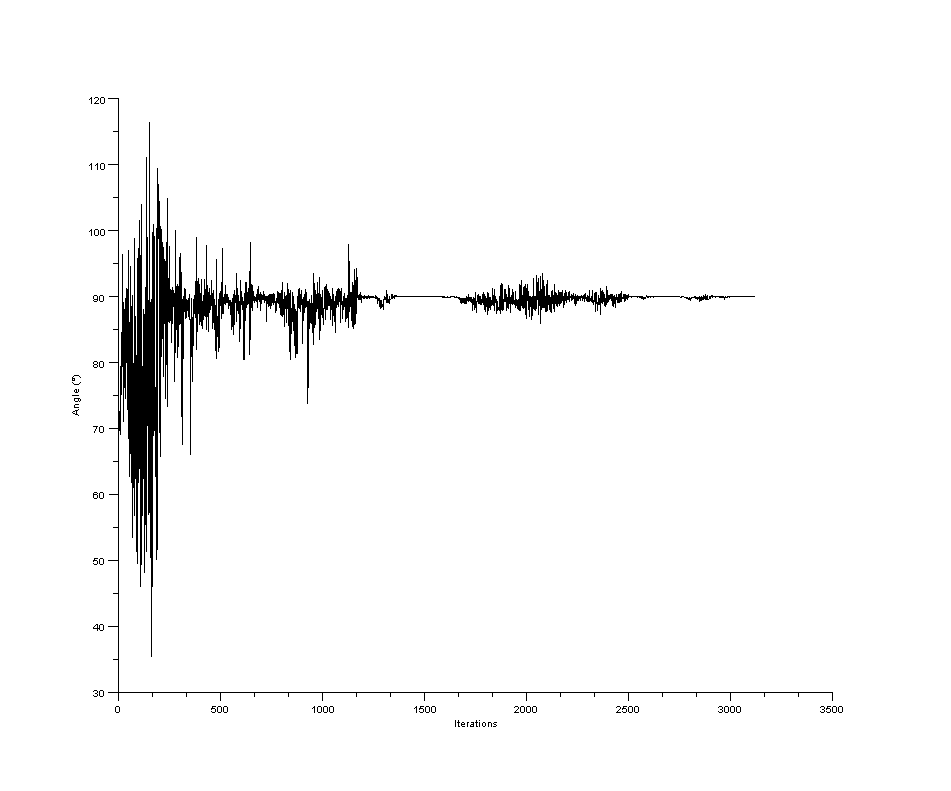
\includegraphics[width=10cm]{torczon_test1_angle.png}
\end{center}
\caption{Nelder-Mead numerical experiment -- Penalty \#1 function --
We see that the angle between the gradient and the search direction
is very close to $90^{\circ}$, especially for large number of iterations.}
\label{fig-nm-numexp-torczon1}
\end{figure}

The numerical experiment shows that the conditioning of the matrix 
of simplex direction has an increasing condition number. This corresponds to the 
fact that the simplex is increasingly distorted.

\section{Conclusion}

The main advantage of the Nelder-Mead algorithm over Spendley et al.
algorithm is that the shape of the simplex is dynamically updated.
That allows to get a reasonably fast convergence rate on badly scaled
quadratics, or more generally when the cost function is made 
of a sharp valley. Nevertheless, the behavior of the algorithm when the 
dimension of the problem increases is disappointing : the more there are 
variables, the more the algorithm is slow. In general, it is expected 
that the number of function evaluations is roughly equal to $100n$.



\clearpage


%% Bibliography

\addcontentsline{toc}{chapter}{Bibliography}
\bibliographystyle{plain}
\bibliography{neldermead}

% Index
\printindex

\end{document}
